% Cover letter using letter.cls
\documentclass[a4paper]{scrreprt} 
%\usepackage{helvetica} % uses helvetica postscript font (download helvetica.sty)
%\usepackage{newcent}   % uses new century schoolbook postscript font 
\usepackage[utf8]{inputenc}
\usepackage[toc,page]{appendix}
\usepackage{graphicx}
\usepackage{amsmath}
\usepackage{eurosym}
\usepackage{cite}
\usepackage{tabularx}
\usepackage{bytefield}
\usepackage{color}
\usepackage{longtable}
\usepackage{tabularx}
\usepackage{url}
\usepackage[bookmarks]{hyperref}
\hypersetup{pdftex,colorlinks=true,allcolors=black}
\usepackage{hypcap}
\usepackage{listings}
\usepackage{color}
% the following commands control the margins:
%\topmargin=-1in    % Make letterhead start about 1 inch from top of page 
%\textheight=8.5in    % text height can be bigger for a longer letter
%\oddsidemargin=0pt   % leftmargin is 1 inch
%\textwidth=6.5in     % textwidth of 6.5in leaves 1 inch for right margin
\title{Implementing a temperature and humidity sensor network for the nEDM
experiment setup}
\author{Wenwen Chen, Rainer Schönberger}
\begin{document}
\maketitle
\tableofcontents
%###############################################################
\chapter{Introduction}
%%%%%%%%%%%%%%%%%%%%%%%%%%%%%%%%%%%%%%%%%%%%%%%%%%%%%%%%%%%%%%%
\section{Background}
\subsection{The neutron electric dipole measurement}
According to the standard model, it is assumed, that neutrons posess a electric dipole moment (EDM)
in the order of $10^{-32}e\cdot cm$. However an extenstion of the standard model already predicts
a dipolemoment in the order between $10^{-26}e\cdot cm$ and $10^{-28}e\cdot cm$. Until now, no
experiment was able to do measurements more precise than $10^{-26}e\cdot cm$\cite{frmexp}.\\
The Neutron EDM (nEDM) experiment at Technische Universitat München is trying to increase the precision
of such a dipolemoment measurement\cite{frmexp}.\\
The experiment uses spin polarized ultracold neutrons, which are guided into two chambers inside a
highly controlled and magnetically shielded environment (see figure \ref{fig:exp}). There, a spin precession measurement according
to Ramsey \cite{ramsey} is performed, which allows it, to get information about the dipole moment of the neutons.
\begin{figure}[h]
\centering
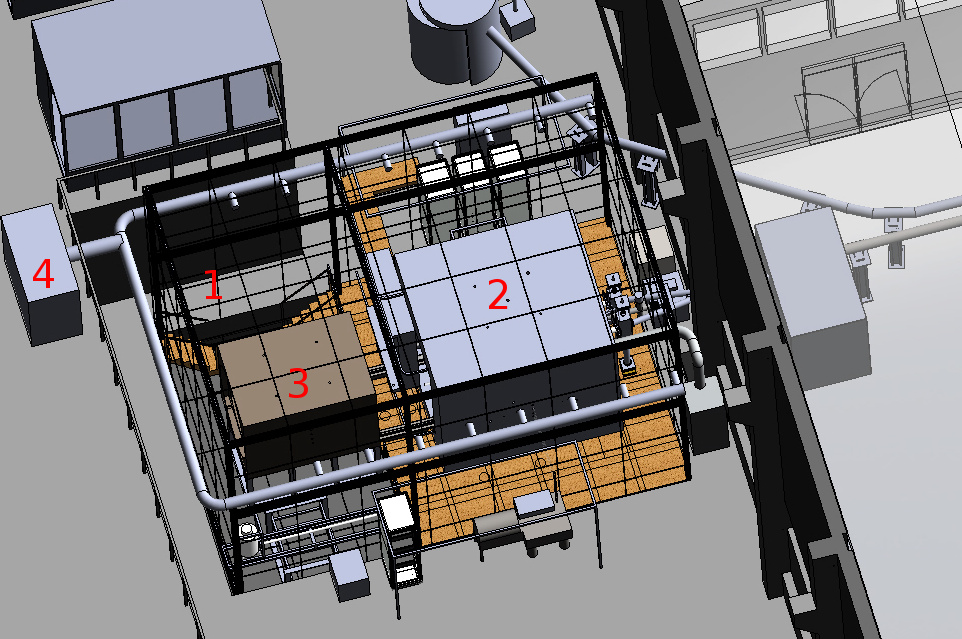
\includegraphics[width=0.87\linewidth]{img/frm3d.jpg}
\caption{Experiment environment. 1: Field cage for magnetic field compensation, 2: Outer magnetic shield, 3: Inner magnetic shield, 4: Air conditioning system.}
\label{fig:exp}
\end{figure}
\subsection{Temperature measurement}
Besides an exactly defined magnetic environment inside the experiment setup, a well defined
environment temperature and humidity is also important for the experiment. Therefore a
air conditioning system is installed to regulate the temperature inside the field cage.
Our temperature sensor network will provide data for the air conditioning system.\\
As a precise homogenous temperature distribution inside the whole field cage is
almost impossible to achieve, our sensor network will provide precise temperature and humidity data. These data can be used to determine if specific physical observations are dependant
on temperature changes in the environment. Also a temperature compensation of measurements
based on environment temperature is possible.
%%%%%%%%%%%%%%%%%%%%%%%%%%%%%%%%%%%%%%%%%%%%%%%%%%%%%%%%%%%%%%%
\section{Features}
Our finished sensor network provides the following features:
\begin{itemize}
  \item Both temperature and humidity sensors can be connected at any
    sensor socket. The sensor type will be automatically detected.
  \item High temperature and humidity accuracy: Temperature sensors
    are calibrated to $\pm 0.1\,\mathrm{K}$ and the humidity
    sensors to $\pm 1.8\,\%\mathrm{RH}$.
  \item A high number of connected sensors is supported.
    Currently 44 sensors are in use, however the system is designed
    to support at least 100 sensors and still be able to fulfill a
    sampling rate of $1\,\mathrm{Hz}$. If the sampling rate is
    allowed to be slower, up to 960 sensors are possible to share
    one ethernet connection.
  \item We achieved a relatively low cost per sensor. The cost per
    sensor module is mostly
    defined by the sensor chip alone, which is about \EUR{7} for a
    precision temperature sensor and about \EUR{20} for a high quality
    humidity sensor (also see section \ref{chap:sensors}). The cost for
    the printed circuit board and required components is less than
    \EUR{4} per board.
  \item Measurement results can be forwarded via TCP/IP to a CouchDB
    server, which is able to record the measurement data from all
    connected sensors.
  \item The system supports a fast sample rate of at least $1\,\mathrm{Hz}$.
  \item Most of the system parameters like sampling rate or database IP addresses
    and insert functions are configurable at runtime.
  \item The sensor network provides a TCP/telnet user interface, for
    controlling and viewing of network parameters. This allows easy configuring
    and debugging of the system.
  \item Plug and Play is supported for adding and removing sensors or even
    control units during runtime.
\end{itemize}
%###############################################################
\chapter{Technology}
%%%%%%%%%%%%%%%%%%%%%%%%%%%%%%%%%%%%%%%%%%%%%%%%%%%%%%%%%%%%%%%
\section{Sensors}\label{chap:sensors}
\subsection{TSIC 506F}
For temperature measurements, we use the TSIC 506F temperature sensor
integrated circuit chip. At a relatively low price of about \EUR{7} per device, it
is able to deliver very high accuracy (see table \ref{tab:tsic}).\\
The temperature is converted to a digital value, which is sent out over a
proprietary one wire protocol variant, called \emph{ZAC-Wire}. The transmission structure can be seen in figure \ref{fig:tsic_transmission}. Details about the ZACwire protocol are described in section \ref{chap:zac}.\\
The temperature $T$ in celsius can be calculated from the received value $T_{dig}$ using
$$T\,[^{\circ} C] = \frac{T_{dig}}{2047} \cdot 70 - 10$$\\
In order to minimize soldering heat, which would influence the calibration, we used the TO92 packaged sensor.\\
For further information about the sensor, and data interpretation, please refer to \cite{tsic} and \cite{tsic2}.
\begin{table}[Hh!]
	\centering
	\begin{tabular}{| r | c |}
		\hline
		Temperature range & $-10\,^{\circ}\mathrm{C}$ to $60\,^{\circ}\mathrm{C}$\\
		\hline
		Calibrated accuracy & $\pm 0.1\,\mathrm{K}$  \\
		\hline
		Resolution & $0.034\,\mathrm{K}$  \\
		\hline
	\end{tabular}
  \caption{TSIC 506F specification \cite{tsic2}}
	\label{tab:tsic}
\end{table}
\begin{figure}[Hh!]
	\centering
	\definecolor{lightgray}{gray}{0.8}
	\begin{bytefield}[endianness=big, bitwidth=2.1em]{10}
		\bitheader{0-9}\\
    \bitbox{1}{ST} & \bitbox{5}{0} & \bitbox{3}{$T_{dig}$[10:8]} & \bitbox{1}{P}\\
    \bitbox{1}{ST} & \bitbox{8}{$T_{dig}$[7:0]} & \bitbox{1}{P}
	\end{bytefield}
  \caption{TSIC transmission structure. The temperature is sent over the wire, with two ZACwire transmissions. P is an even parity bit. ST is the start bit \cite{tsic}.}
	\label{fig:tsic_transmission}
\end{figure}
\subsection{HYT271}
For humidity measurement, we use the HYT271 sensor. At a price of about \EUR{20} per device it is significantly more expensive than the temperature sensors, however it delivers precice and temperature compensated humidity measurements. 
The humidity value rH in percent can simply be calculated from the received value $\mathrm{rH}_{dig}$ using
$$\mathrm{rH}\,[\%] = \frac{100}{2^{14}} \cdot  \mathrm{rH}_{dig}$$\\
In addition, the temperature can also be read out and calculate using 
$$T\,[^{\circ} C] = \frac{165}{2^{14}} \cdot  T_{dig} - 40$$\\
Table \ref{tab:hyt} lists the specified sensor characteristics.
\begin{table}[Hh!]
	\centering
	\begin{tabular}{| r | c | c |}
		\hline
    &Temperature & Humidity\\
		\hline
		\hline
    Range & $-40\,^{\circ}\mathrm{C}$ to $125\,^{\circ}\mathrm{C}$ & $0\, \mathrm {\%RH}$ to $100\, \mathrm {\%RH}$\\
		\hline
    Calibrated accuracy & $\pm 0.2\,\mathrm{K}$ & $\pm 1.8\, \mathrm {\%RH}$   \\
		\hline
    Resolution & $0.015\,\mathrm{K}$ & $\pm 0.03\, \mathrm {\%RH}$ \\
		\hline
	\end{tabular}
  \caption{HYT271 specification \cite{hyt}}
	\label{tab:hyt}
\end{table}\\
Communication with the sensor is done via I2C. Thereby measurements can be initialized via addressing the sensor and sending a write bit. The result of a measurement can be received by initializing an I2C read transfer, followed by reading the measurement data. Figure \ref{fig:hyt_transmission} shows the format of received measurement data. The second status bit, the stale bit, sent at the beginning, gives information, whether a new measured value is ready after the last readout. The reception of data may be aborted, by the I2C master after every byte, if not all data is needed.
\begin{figure}[Hh!]
	\centering
	\definecolor{lightgray}{gray}{0.8}
	\begin{bytefield}[endianness=big, bitwidth=2.1em]{8}
		\bitheader{0-7}\\
    \bitbox{2}{Status} & \bitbox{6}{Humidity [13:8]}\\
    \bitbox{8}{Humidity [7:0]}\\
    \bitbox{2}{\color{lightgray}\rule{\width}{\height}} & \bitbox{6}{Temperature [13:8]}\\
    \bitbox{8}{Temperature  [7:0]}
	\end{bytefield}
  \caption{HYT271 transmission structure. The humidity value and temperature value each consist of 14 bits. The two bits, marked with gray color, before the temperature value are not used \cite{hyt2}.}
	\label{fig:hyt_transmission}
\end{figure}\\
For further information about the sensor, and data interpretation, please refer to \cite{hyt}, \cite{hyt3} and \cite{hyt2}.
%%%%%%%%%%%%%%%%%%%%%%%%%%%%%%%%%%%%%%%%%%%%%%%%%%%%%%%%%%%%%%%
\section{Protocols}
In this section, the mainly used low level protocols for measuring and data forwarding will be introduced shortly. 
\subsection{ZACwire}\label{chap:zac}
ZACwire is a proprietary one wire comminucation protocol, developed
by IST AG. ``One wire'' means that only one data line is needed.\\
Each bit is represented by
different duty cycles of the waveform within the bit time $T_b$.
Every normal bit starts with a falling edge. At the beginning
of each transmission, a start bit with a duty cycle of 50\% is
transmitted. From this start bit, the bit time $T_b$ for the
transmission can be extracted. 
If the bus is 75\% high within the bit time $T_b$ the bit `1' is transfered, otherwise bit `0'. 
If the bus is high for a time $>T_b$
the transmission ends, this is called a Stop bit. Figure \ref{fig:zac}
shows the four different wafeform types, of which a ZACwire signal can be
composed. Figure \ref{fig:zacexample} shows an example
transmission. For further information see \cite{zac}.
\begin{figure}[Hh!]
	\centering
	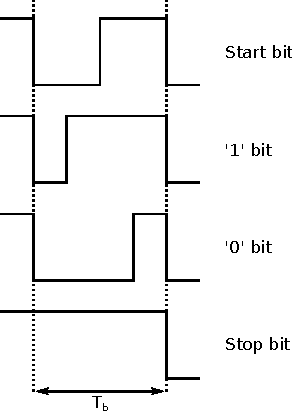
\includegraphics[width=0.3\textwidth]{img/zac_bits.pdf}
	\caption{ZACwire protocol signal interpretation}
	\label{fig:zac}
\end{figure}
\begin{figure}[h]
	\centering
	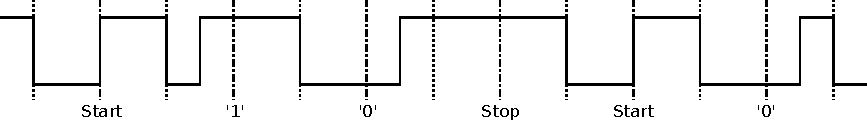
\includegraphics[width=0.9\textwidth]{img/zac_example.pdf}
	\caption{ZACwire protocol example}
	\label{fig:zacexample}
\end{figure}
\subsection{I2C}
I2C is a bus protocol, which specifies the physical layer, as well as an arbitration and addressing layer. The protocol is a two wire protocol and allows communication between multiple bus participants.\\
Transmissions are done over two transmission lines SCL and SDA, which
are pulled to logical high voltage level by pullup resistors (see
figure \ref{fig:i2c}). Each transmission is controlled by a device
in master mode, which provides a clock by controlling the SCL line.\\
A transmission is surrounded by a START and a STOP bit, which are code violations.\\
At the beginning of a transmission, the master first transmits an
address to the bus, addressing one or all connected devices which
are in slave mode. After that a data direction bit is sent to the
bus, which defines the slave behavior: read or write. If the direction bit specifies a write, all addressed slave devices read bits from the bus at every 
clock cycle, the SDA line stays under control of the master. If the
direction bit describes a read, the slave should take control over
the SDA line and transmits bits at every clock cycle.\\
The Slave is allowed to take control over the SCL line at any time
by pulling it low. this is called clock extenstion, and signals the
master to not proceed transmitting or receiving data.
The full I2C specification can be found in \cite{i2c}.
\begin{figure}[Hh!]
	\centering
	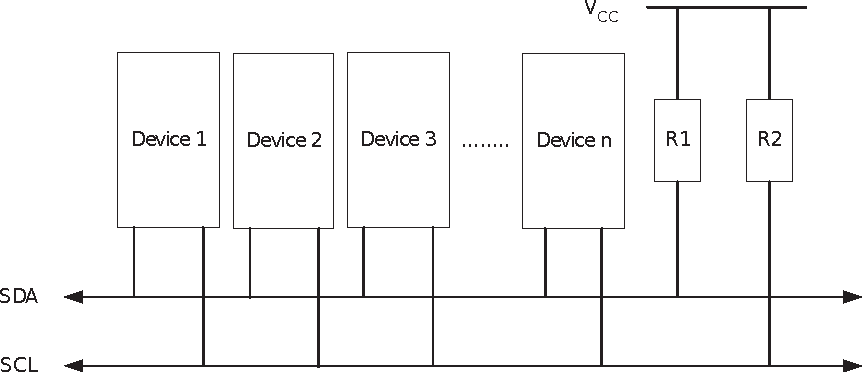
\includegraphics[width=0.7\textwidth]{img/i2c.pdf}
  \caption{I2C logical bus structure. Source \cite{i2c}.}
	\label{fig:i2c}
\end{figure}
\subsection{RS485}
RS485 is a transmission line standard, which specifies differential line communication over twisted pair cables.
It allows very long distance communication of up to 1 kilometer with high noise immunity and reduced noise emission.\\
Figure \ref{fig:rs485} illustrates the working principle of the protocol.
The encoder transforms a single bit line DI into two separate lines A and B.
If DI is high, the output voltage at line A ($V_{OA}$) will be bigger than at line B ($V_{OB}$).
If the input voltage at DI is low, $V_{OB}>V_{OA}$ holds.\\
A detailed description of the protocol and its implementation can be found in \cite{rs485}, \cite{st485} and \cite{st485appnote}.
\null
\vfill
\begin{figure}[htbp]
	\centering
	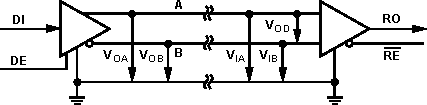
\includegraphics[width=0.65\textwidth]{img/rs485.pdf}
  \caption{RS485 encoding/decoding - Logical structure. Source: \cite{rs485}.}
	\label{fig:rs485}
\end{figure}
%%%%%%%%%%%%%%%%%%%%%%%%%%%%%%%%%%%%%%%%%%%%%%%%%%%%%%%%%%%%%%%
\section{Toolchain}
\subsection{KiCad}
To design schematic circuit diagrams, as well as printed multilayer circuit boards, we used the open source EDA suite KiCad\footnote{http://www.kicad-pcb.org}. Most of the schematic and footprint components, were designed by ourselfes and can be found in the project git repository.\\
The finished board files were exported to the Gerber / Echelon file format and sent to Fischer Leiterplatten\footnote{http://www.fischer-leiterplatten.de} for production.
\subsection{ISP programming}\label{chap:isp}
To upload the compiled code and to configure the microprocessors, we used the USBasp programmer in combination with the avrdude software.\\
As we needed to access the fuse bytes of the arduino too, which was not possible with the arduino bootloader, we also use the ISP header on the Arduino board for programming. The arduino bootloader was removed. Hence it is not possible anymore, to programm the arduino with the arduino software suite, without reinstalling the bootloader.\\
\textbf{Note} that the arduino ISP header is not compatible with the one, provided by the USBasp programmer. A mechanical adapter or individual cabling is required. 
Figure \ref{fig:isp} shows the pin asignments of the different ISP headers.
\begin{figure}[htbp]
	\centering
	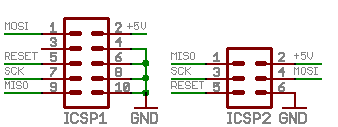
\includegraphics[width=0.35\textwidth]{img/isp.png}
  \caption{ISP connector pin asignments. Left: 10 pin version (used by USBasp, and on our boards), right: 6 pin version (as used on arduino boards). Source: \cite{micronet}.}
	\label{fig:isp}
\end{figure}
\subsection{USART for debugging}
For convenient debuging, we added a USART header on each board with a microcontroller. 
These pins are directly connected to the hardware USART unit of the microconteoller.\\ 
\textbf{Note} that the signal level on this header is TTL and is not compatible with the RS232 standard. It is possible to connect the boards to a PC, using either an external signal level converter from TTL to RS232, or a direct USB to USART TTL converter.\\
In every software component, we set the \emph{stdout} file descriptor, to point to a USART file, implementing writing data to the USART line.
Hence standard file handling functions like \emph{printf} or \emph{puts} can be used for printing debugging information.\\
To read and write data at the PC side, software like \emph{screen} or \emph{picocom} may be used. The default baud rate is 9600bps.
\subsection{Build process}
To build and upload the code the following software and libraries are required:\\
Tools:
\begin{itemize}
  \item avr-gcc
  \item avr-objcopy
  \item avrdude or other ISP programming software
\end{itemize}
Libraries:
\begin{itemize}
  \item avr-libc
  \item Arduino ethernet library (only for ethernet board)
  \item Arduino core library (only for ethernet board)
\end{itemize}
We use the make build environment. The Makefiles in each software directory contain instructions on how to build and upload the software to the microcontroller, using the following rules:
\begin{description}
  \item[make clean] Clears the build directory.
    %FIXME make makefile clever for use/create build folder
  \item[make] Compiles and links the source code to the elf and intel hex binary format. Also a EEPROM image is generated in intel hex binary format. The output directory for binary files will be \emph{./build/}.
  \item[make fuse] Configures the controller, to use the right system clock source, burnout detection and eeprom persistency settings.
  \item[make eeprom] Uploads the EEPROM image to the controller.
  \item[make upload] Uploads the compiled software to the microcontroller, using avrdude. By default the usbasp programmer is selected.
\end{description}
For a first time build and upload, the above order should be respected. After the initial upload, fuses and eeprom should not be touched everytime, the software changes.\\
To be able to find the Arduino library root path, the \emph{ARDUINO\_PATH} environment variable should be set to the Arduino installation directory. This for example is the path to the cloned Arduino git reporitory.\\
\textbf{Note}, that the Makefiles in the current version, do not automatically search for file dependancies, hence a make clean should be executed, after every change in not explicitly specified files, namely every non .c or .cpp file.

%###############################################################
\chapter{Implementation}
%%%%%%%%%%%%%%%%%%%%%%%%%%%%%%%%%%%%%%%%%%%%%%%%%%%%%%%%%%%%%%%
\section{Logical design}
Our network architecture is structured into 3 parts (see figure \ref{fig:topo}).
For each part, we developed a different kind of device. The job of each part
is described in the following:
\begin{figure}[Hh!]
	\centering
	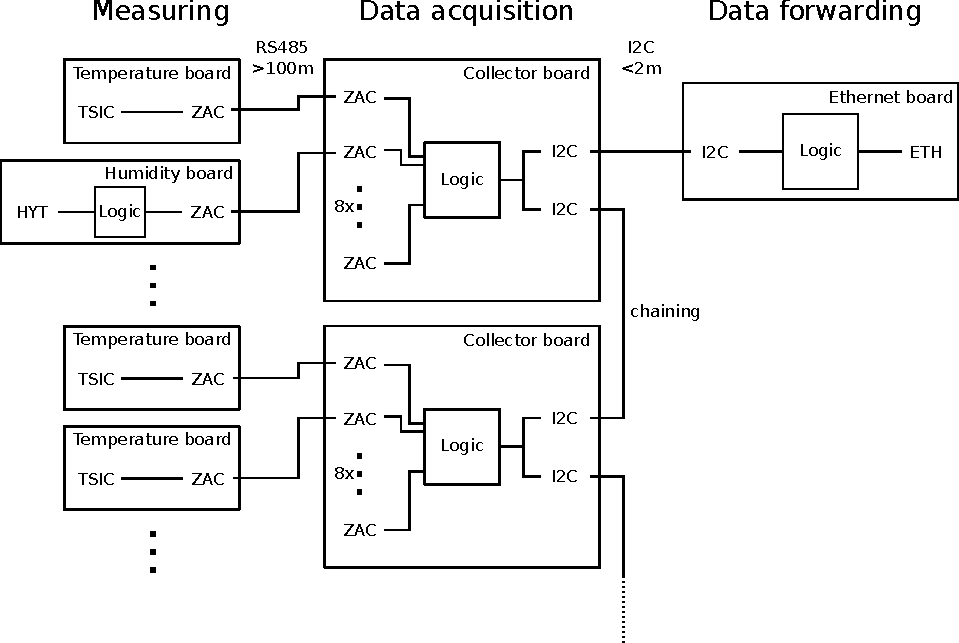
\includegraphics[width=0.9\textwidth]{img/plan2.pdf}
	\caption{Network topology, showing the different devices in the network.}
	\label{fig:topo}
\end{figure}
\begin{description}
  \item[Measuring]\hfill \\
    Sensors do periodic measurements. The results are transmitted,
    using an unified protocol. We used ZACwire, as the unified
    protocol, as in our application we have more temperature sensors,
    which natively speak ZACwire, than humidity sensors. Hence no
    protocol conversion will be required for the majority of the
    sensor boards. 
    Using RS485 as a physical layer protocol, the range of the
    ZACwire signal has been extended with a improved noise behavior.
  \item[Data acquisition]\hfill \\
    At this part of the network, the ZACwire signal from the sensors
    is interpreted and buffered. The measurement data is then
    provided over an I2C interface.\\
    In our implementation, we support sampling of up to 8 Sensors
    per collector board. To increase the numbers of sensors in the
    network, multiple collector boards may be connected to the I2C
    bus, using the I2C chaining connectors. With this technique,
    the network theoretically may consist of up to
    $120\cdot 8 = 960$ sensors\footnote{Eight I2C addresses are reserved}.
  \item[Data forwarding]\hfill \\
    The forwarding part controls the data aquisition part of the
    network and provides an interface to IP networks. Data can be
    forwarded to a couchDB database on the internet. Furthermore, the network 
    is configurable via an telnet/netcat terminal user interface.
\end{description}
%%%%%%%%%%%%%%%%%%%%%%%%%%%%%%%%%%%%%%%%%%%%%%%%%%%%%%%%%%%%%%%
\section{Sensor boards} \label{chap:sensorbrd}
\subsection{Temperature board} \label{chap:tempbrd}
The temperature board consists of the TSic506F sensor and
complementary circuitry. The ZACwire signal is transformed to the
RS485 electrical layer, using a ST485 integrated circuit. The board
provides a RJ45 socket,  over which the required supply voltage of 5V
should be provided, and the two differential signal outputs can be
received. The schematic diagram can be seen in figure
\ref{fig:schem_temp}.\\
Care was taken, when soldering the temperature sensor, to minimize
heat transfer to the chip. We did this by soldering each pin for a
maximum time of 2 seconds, We also tried to keep the total time spent
for soldering all 3 pins less than 10 seconds. After soldering, we
immediately blowed cold air to the pins and the chip itself.\\
Figure \ref{fig:pcb_temp} shows the printed circuit board (PCB) schematic
and figure \ref{fig:soldered_temp} the not completely soldered
temperature board. 
In order to reduce the influence of heat from the other electronic
components, the temperature sensor is placed far away from the others
and PCB the traces to the temperature sensor are thin and guided through
a narrow neck.
\subsection{Humidity board}
The hardware structure is similar to the temperature board, described in section \ref{chap:tempbrd}. However, as the HYT271 sensors use I2C for
communication, we added a microcontroller to repediately poll the sensor for current measurement results and send the data out using a software
implementation of the ZAC wire protocol. Therefore we also placed an ISP socket, a debugging adapter, a reset switch and two LEDs onto the board, which makes it
slightly bigger than the temperature board. The schematic can be seen in figure \ref{fig:schem_hum}.\\
The design of the pcb (see figure \ref{fig:pcb_hum}) is also similar to the temperature board. 
\subsubsection{ZAC encoding}
The most easy method to generate a ZAC encoded signal is to set a pin high, then use busy-wait delay loop (\texttt{\_delay\_us()}) to wait a certain time interval. After that set the pin to low. 
But the timing of this method is not very exact (more than 6 $\mu$s inaccuracy according to experience). Hence we decided to use a timer to achive a higher timing accuracy. \\
We have used the following timer features, which are triggered on compare match: 
\begin{itemize}
  \item Clear timer, when the timer counter matches the output compare register value. This is the so called ``CTC mode'' of the timer.
  \item Toggle an output pin if a compare match occurs. It will be also possible to explicitly set the pin high or low.
  \item Excute an interrupt handler on compare match. This allows us to change the value of the output compare register on demand.
\end{itemize}
Figure \ref{fig:zac_encoding} shows an example of the ZACwire signal encoding process.\\
\begin{figure}[Hh!]
	\centering
	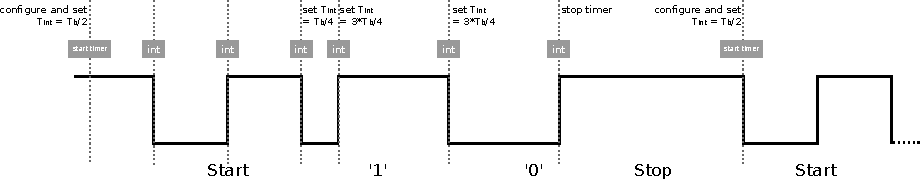
\includegraphics[width=\textwidth]{img/zac_encoding.pdf}
	\caption{ZACwire signal encoding processing example.}
	\label{fig:zac_encoding}
\end{figure}
We keep the output pin high, when there is nothing to do.
If a measured value is ready to be sent, the timer will be configured to enable the above described features and the output campare register will be set to half of the defined bit time for sending a start bit.
After that, the output compare register will be set to $\frac{T_{b}}{4}$ or $\frac{3}{4}T_{b}$ according to the sending bit.
After the last bit is sent, the output pin will stay high, which indicates a stop bit. 
When a newly measured value is ready again, the whole procudure will be excute again.
\\
For detailed usage description of the microprocessor timer, please read the corresponding datasheet. For the microprocessor ATmega88P, which we used, see \cite{atmega88}. 
\subsubsection{Cyclic redundancy check (CRC)}
In order to detect errors after a long distance transmission, 
We attach an 8-bit CRC checksum for every block of measured values before sending the data out. \\
CRC is a common method for error-detecting in digital networks and is based on the theory of polynomial division. 
In the galois field of two elements, GF(2),
an n-bit checksum is the remainder of the division between data, shifted n bit to the left, and a (n+1)-bit polynomial as the divisor.
Because the polynomial division in GF(2) is equivalent to an iteration of the bitwise XOR, a checksum can be computed in the following way:
The divisor is at first shifted to the leftmost side of the input data block and computed XOR with the first (n+1) bits.
Then the rest of the unchanged input is appended to the result and becomes the new input to do the same XOR calculation with the divisor again.
If the result is zero, the divisor will be shifted to the first bit `1' and XORed with the (n+1) bits, starting with the bit `1'. 
The XOR calculation will be repeated until no rest bits exist to attach and the n bits remainder then is the wanted CRC checksum.
An example of the calculation of a 4-bit checksum to the polynomial divisor 10011 (0x13) using this algorithm will be shown below:
\definecolor{backcolour}{rgb}{0.95,0.95,0.92}

\lstdefinestyle{mathstyle}{
    backgroundcolor=\color{backcolour},   
    basicstyle=\scriptsize\ttfamily,
    breakatwhitespace=false,         
    breaklines=true,                 
    captionpos=b,                    
    keepspaces=false,                                 
    showspaces=false,                
    showstringspaces=false,
    showtabs=false,                  
    tabsize=2
}
\lstset{style=mathstyle}
\begin{lstlisting}[xleftmargin=25pt, xrightmargin=25pt,framexleftmargin=10pt,framextopmargin=10pt, framexbottommargin=10pt]
1101 1001 1010 0011 0000  <-- input data block, shifted 4 bits to left 
1001 1                    <-- polynomial divisor
------------------------
 100 0001 0100 0011 0000  <-- result of the frist XOR round
 100 11
 -----------------------
     1101 0100 0011 0000
     1001 1
     -------------------
      100 1100 0011 0000
      100 11
      ------------------
                 11 0000
                 10 011
                 -------
                  1 0110
                  1 0011
                  ------
                     101 <---remainder, the checksum
\end{lstlisting}
For checking the correctness of received data, the division of received data and the same polynomial is repeated.
If the remainder is not equal zero, some error of the transfered data is detected, otherwise no error is found.
But that does not mean, no error exists.
It might happen, that the change of some bits accidentally leads to a zero remainder. However, the probability of such detectable error is very low.\\
The polynomial, which we use, is the standard CRC-8 for 1-wire bus systems: 100110001(0x131).
%%%%%%%%%%%%%%%%%%%%%%%%%%%%%%%%%%%%%%%%%%%%%%%%%%%%%%%%%%%%%%%
\section{Collector board}
The collector board decodes the ZAC protocol and provides an I2C interface
for users, to read out temperature, as well as humidity values of connected sensors.
Care was taken, to ensure a response time of $<1\,\mathrm{s}$.
\subsection{Hardware}
The schematic diagram can be seen in figure \ref{fig:schem_collect}. The hardware consists of the following main components:
\begin{description}
  \item[Microprocessor:]\hspace{1cm}\\
    To do all protocol conversion tasks, we used an Atmel Atmega88PA
    microcontroller, running at a clock speed of $20MHz$. The clock
    is generated, using an external crystal oscillator.\\
    The Atmega microconteoller provides a variety of useful features
    like asynchronous timers, pin change interrupts on every GPIO (General Purpose Input/Output)
    pin, hardware support for the I2C protocol and integrated EEPROM
    storage (Datasheet: \cite{atmega88}).\\
    We connected the sensors in two groups, so that we are able to
    receive two independent interrupts for two sensors in different
    groups.
  \item[I2C connection:]\hspace{1cm}\\
    The board provides two 6-pin I2C pin headers (P3 and P4 of the schematic diagram in figure \ref{fig:schem_collect}), which
    provide connection to the I2C bus, as well as an optional 5V
    power line (Vi2c). The two headers are connected in parallel,
    so they can be used for chaining multiple collector boards.\\
    The board also has integrated I2C pullups, which can be enabled
    using the switch SW2 (see figure \ref{fig:schem_collect}), in case the I2C master does not provide
    pullups.
  \item[Sensor connection:]\hspace{1cm}\\
    The individual sensors are connected via an eight-port RJ45
    socket header. Shielding of the RJ45 sockets is connected to
    board ground. The signal of each sensor is first interpreted
    by an RS485 transceiver and afterwards directly provided to a
    microcontroler GPIO pin. As this is the receiving side, we also
    had do add impedance matching circuitry. We chose to implement
    a power saving AC-termination solution, as suggested in \cite{st485appnote, rs485}.
    To bring the output level of each transceiver to a defined state,
    when no sensor is connected, we use pullup resistors on the
    input side. Optionally the board and shield ground can be wired to
    the screw pad P2 (see figure \ref{fig:schem_collect}) for a connection with the casing. This is done by
    placing the 0 Ohm resistor R34.
  \item[Developer interface:]\hspace{1cm}\\
    The microcontroller can be programmed with any AVR In System
    Programmer, using the standard ISP header (P8 in figure \ref{fig:schem_collect}).\\
    For debugging code, we also added a USART pin header (P1 in figure \ref{fig:schem_collect}), which
    allows serial communication with the microcontroller. 
    \\
    \textbf{Note}, when connecting the chip to a PC, as the logic
    levels of our board are 5V TLL and hence are not compatible
    with the RS-232 logic levels, used by most PCs. We suggest to use
    a USB to USART TLL converter or a logic level converter.
  \item[Power source:]\hspace{1cm}\\
    We provide multiple ways to supply power to the collector board.
    \begin{itemize}
      \item Direct 5V input/output (P7 or P9 in figure \ref{fig:schem_collect})
      \item Use the 5V supply voltage, provided via the I2C bus
      \item Unregulated input (7V..25V). The onboard LM7805 linear
        regulator, will convert the voltage to 5V.
    \end{itemize}
    Using the pin header K1, which is marked in figure \ref{fig:schem_collect}, it is possible to select suitable
    power inputs.\\
    Example 1: If the board should get power over I2C, pins 1 and 2
    should be shorted.\\
    Example 2: If the board should get power from the on board
    regulator, and also provide power to the I2C bus, all three pins
    should be shorted.
\end{description}
\subsection{ZAC decoding}
AVR controllers do not have hardware support for decoding the ZAC one wire
protocol (protocol definition is explained in chapter \ref{chap:zac}). Hence we
implemented a software decoder. However our implementation
does not follow the method suggested by \cite{zac} because of timing reasons.\\
To decode one ZAC protocol sensor, we use the pin change interrupt (PCINT) of the pin, connected to the sensor, and
one 8 bit timer, the corresponding timer overflow interrupt.
\paragraph{Pin change Interrupt:} On every pin change interrupt, the following actions are executed:\\
%FIXME redudancy of every time
Every time:
\begin{itemize}
	\item The current current value is stored to a temporary variable $T_{timer}$, to be able to still access it later.
	\item The timer is reset.
	\item If the timer is not jet running, it is started now.
\end{itemize}
On a falling edge:
\begin{itemize}
        % FIXME what is Tcrit, it is not cleared at the first usage, und the explain after that is also not that understandable!
	\item If $\left|T_{low} - T_{timer}\right| < T_{thresh}$ with a constant $T_{thresh} << T_{crit}$, we
		have observed a start bit.\\
		We now update the critical sampling time\footnote{$T_{crit} = 0.5\cdot(T_{timer} + T_{low})$ would
		be more accurate, but would consume more time to calculate.}: $T_{crit} = T_{timer}$.
\end{itemize}
On a rising edge:
\begin{itemize}
	\item The current timer value is stored as $T_{low}$. If we already observed a falling edge, this
		represents the time, the signal was low.
	\item If we already have seen a start bit, we now sample a data bit\footnote{Note, that a repeated
            % FIXME how to avoid to read the second start bit into measured data
		start bit would also be sampled as a data bit with an unpredictable value.}:\\
	$\mathrm{bit} = \begin{cases} 1 & \text{if } T_{timer}<T_{crit} \\ 0 & \text{else}\end{cases}$
\end{itemize}
\paragraph{Timer overflow Interrupt:} The timer is configured in a way, that an overflow will occur after
the timer is running without a reset for $T_{ovf}$, with $T_{bit} < T_{ovf} < 100\,\mathrm{ms}$. Hence
the interrupt will occur, after a completed transmission and before the start of the next transmission.\\
%FIXME how to check, what is the criteria
After a overflow occurs, we check, if we received a whole transmission. If this is the case, we disable
interrupts and stop the current measurement. Otherwise we reset the receive buffer and wait for the
next transmission to begin.
%\paragraph{Starting a measurement:} 
\\[0.6cm]
At the beginning of each meassuring process, the following is executed:
\begin{itemize}
	\item $T_{crit}$ is set to the maximum value.
	\item $T_{low}$ is set to the minimum value. This will ensure, that we do not
		accidentally recognize the first falling edge as a start bit.
	\item The receive buffer is reset.
	\item Interrupts are enabled.
\end{itemize}
%\paragraph{}
Our algorithm is not able to see stop bits correctly, if $T_{ovf}$ is configured badly.
However in our case we deliberately configured $T_{ovf}$ to be bigger that the maximum
high time in case of a stop bit.
This allows us to only see the end of the complete transmission, as a TSIC sensor also
sends an useless stop bit after the first 9 bits.\\
%\paragraph{}
As we have up to 8 sensors connected to the Atmega88, we have to do one measurement after another.
As one sample of a measurement takes $>100\,\mathrm{ms}$ we would run
into problems reaching the desired sampling rate of $>1\,\mathrm{Hz}$.
Our approach is to sample two sensors at the
same time, using a second 8 bit timer. Our interrupt handler for the ZAC protocol decoding are not interruptable.
Hence, incomming interrupts are delayed for the runtime $t_e$ of currently executed interrupts.
If we have interrupts active for two sensors at the same time, the controller might see a delayed signal.
Figure \ref{fig:zactiming} illustrates this problem:
\begin{figure}[Hh!]
	\centering
	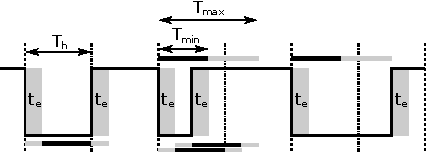
\includegraphics[width=0.7\textwidth]{img/zac_timing.pdf}
	\caption{ZAC protocol worst case timing. The grey shaded areas illustrate the potentially delayed vision
	of a microcontroller due to interrupt latency.}
	\label{fig:zactiming}
\end{figure}
\\
When sampling the start bit we get an error for our critical time $T_{crit}$:
$$T_{min} := T_h - t_e < T_{crit} < T_h + t_e$$
When using $T_{crit}$ to determine a bit value, we are again influenced by the possibly delayed preceeding falling edge. We get:
$$T_{min} < T_{crit}' < T_h + 2 \cdot t_e =: T_{max}$$
In other words, $T_{min}$ is the time, starting from a real falling edge,
before which the controller will not sample the bit. $T_{max}$ is the time,
starting from a real falling edge, after which the controller will not sample
the bit anymore.\\
In order to reliably detect 1s and 0s, our algorithm will only work correctly, if
$$T_{min} > 0.5\cdot T_h + t_e$$
or
$$T_{max} < \frac{3}{2}\cdot T_h\text{.}$$
Both inequations simplify to
$$t_e < \frac{1}{4}\cdot T_h\text{.}$$
According to \cite{zac}, the nominal value for $T_h$ is $\frac{125}{2}\,\mu\mathrm{s}$. Hence our error due to
interrupt latency has to be smaller than $15.625\,\mu\mathrm{s}$.\\
As the microcontroller runs at a clock speed of $20\,\mathrm{MHz}$, we have to complete previous interrupts,
start the interrupt handler of the new interrupt and sample the current timer value within 332 clock cycles,
to not harm the above limit on the error.\\
We implemented a simple branch aware Worst Case Execution Time (WCET) analyzer for the AVR instruction set.
It is able to calculate the maximum execution time of individual sections in the compiled code\footnote{\textbf{Note} that,
whereas branches are considered, only branches to addresses in the future are handled correctly. Loops i.e.
branches to already executed code cause undefined, possibly non terminating behaviour of the analyzer. As our code
does not contain loops, this did not cause problems and loop handling was not implemented.}. Figure \ref{fig:wcet}
shows the WCET analyzer output for the Pin change interrupt handler. The worst case execution time for the total
handler is $100$ cycles. The timer interrupt handler takes less than $50$ cycles to complete. For a complete analysis one
additionally has to consider the time for jumping to the interrupt handler ($<20$ cycles) and the time we need to read out the
timer value in the new interrupt handler ($<29$ cycles). This gives us a total latency of less than $199$ clock
cycles, which is well within the allowed range.
\begin{figure}
	\centering
	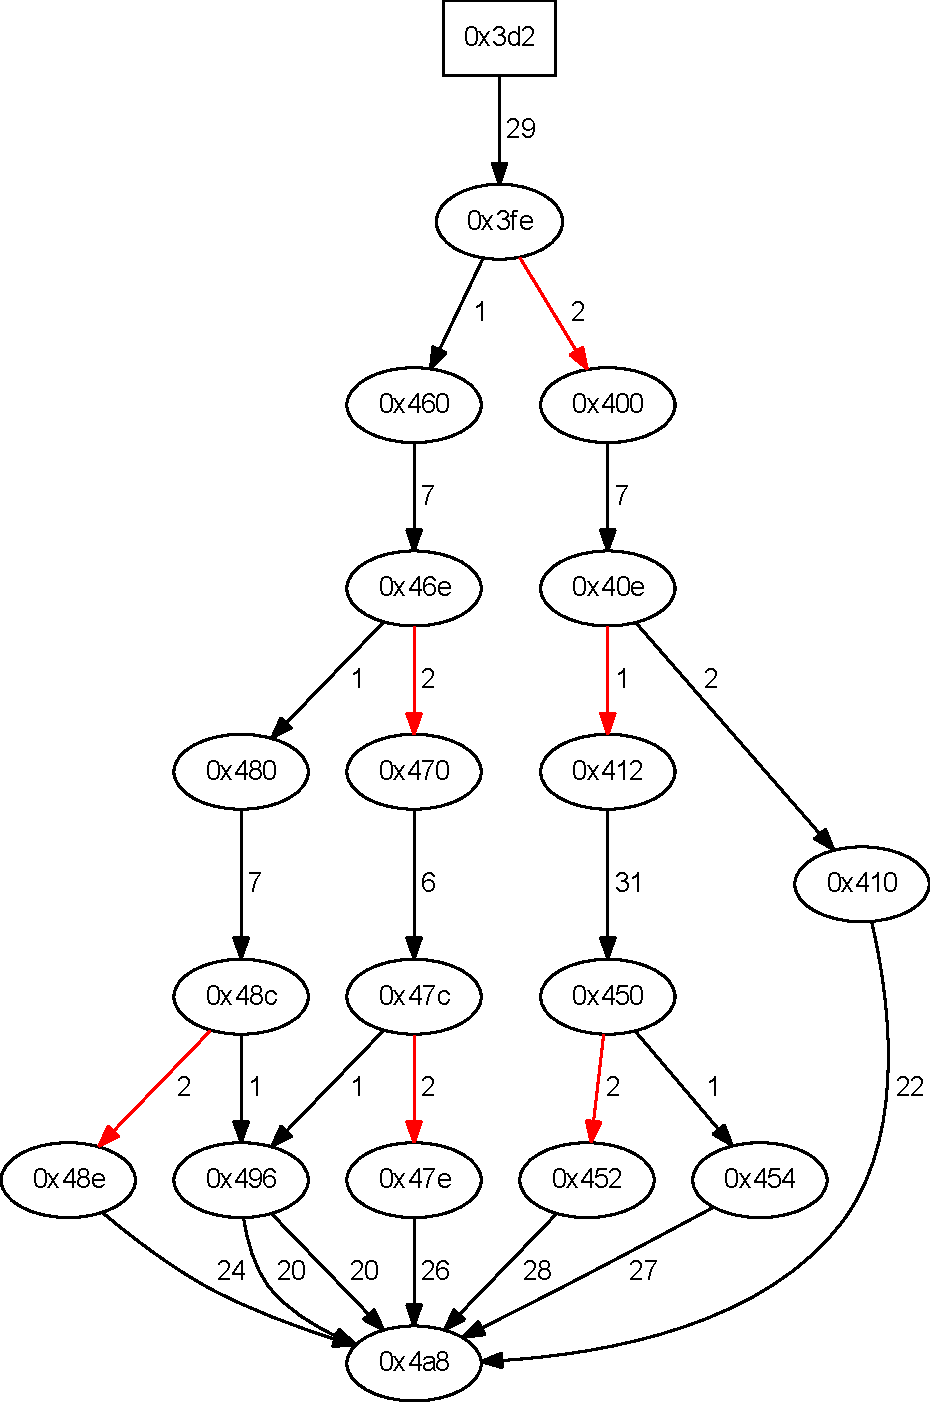
\includegraphics[width=0.5\textwidth]{img/wcet/vector_4.pdf}
  \caption{Branch aware WCET analysis of the Interrupt handler for vector\_4 (Pin change interrupt).
  Nodes represent program addresses, arrows represent branches. Red arrows point to the branch with the
highest execution time. The values near the arrows represent the execution time from the previous node's
address to the instruction causing the branch.}
	\label{fig:wcet}
\end{figure}
\subsection{I2C interface}
Communication with the collector board is done via I2C (Two Wire Interface). Thereby the board acts as an
I2C slave, extending the clock, if it is currently not able to process incomming data.
This is especially used while a measurement is in progress: As soon as new data byte arrives,
it is buffered and the clock will be extended, signalling to the master, that no further data should be sent or received.\\
If a write request (SLA+W) is sent, the following data is interpreted as a command. A list of implemented commands is given
in table \ref{tab:i2c}. The collector board reacts to the general call address 0. This makes it possible to trigger a measurement
on multiple boards, using only one I2C transmission.
% FIXME really without knowing the old one?
Also the own I2C address can be set to a new value without knowing the old one.\\
If a read request (SLA+R) is sent, the packet array from the last completed measurement will be sent out, starting with sensor 0.
For details about the packet format see chapter \ref{chap:packet}. Not all packets have to be received, as soon as a STOP bit is
received, the transmission is aborted. A new read request will again trigger the transmission of data starting at sensor 0.
\begin{table}[Hh!]
	\centering
	\begin{tabularx}{\textwidth}{ | c | c | c | X | }
		\hline
    Name & Value & Parameters & Action\\
		\hline
		\hline
    START\_MEASUREMENT & 0x01 & --- & All 8 sensor values will be
    captured as soon as the STOP bit is received. If during
    measurement
		the slave is addressed again, the I2C clock will immediately be extended until the measurement is complete, blocking the whole I2C bus.\\
		\hline
    SET\_ADDRESS & 0x02 & address & The own I2C address will be updated with the 1 byte value following the command. The address should
        % FIXME 42????
		be in the range from 8 to 112. The default address is 42\\
		\hline
        % FIXME parameter not just number!!!
    LED\_ON & 0x03 & number & The LED with the given number will be turned on.\\
		\hline
    LED\_OFF & 0x04 & number & The LED with the given number will be turned off.\\
		\hline
	\end{tabularx}
	\caption{List of implemented I2C commands}
	\label{tab:i2c}
\end{table}
\subsection{Measurement packet format}\label{chap:packet}
After data was received via the ZAC-Wire protocol, it is interpreted and converted to a convenient packet format, suitable for
redirection via I2C. Figure \ref{fig:packet} shows the structure of a packet.
\begin{figure}[Hh!]
	\centering
	\definecolor{lightgray}{gray}{0.8}
	\begin{bytefield}[endianness=big, bitwidth=2.1em]{8}
		\bitheader{0-7}\\
		\begin{rightwordgroup}{Header}
			\bitbox{2}{type} & \bitbox{3}{\color{lightgray}\rule{\width}{\height}} & \bitbox{1}{c} & \bitbox{2}{error}
		\end{rightwordgroup}\\
		\begin{rightwordgroup}{Payload}
			\wordbox{2}{Temperature}\\
			\wordbox{2}{Humidity}
		\end{rightwordgroup}\\
		\wordbox{1}{CRC-8}
	\end{bytefield}
  \caption{Packet format of a measurement. The whole packet is 6 bytes long}
	\label{fig:packet}
\end{figure}
Each packet's integrity is protected by a CRC checksum and consists of the following fields:\\
\begin{description}
	\item[\textbf{type}] \hfill\\
        This field pecifies the type of the sensor, which supplied the data. Currently implemented values are 0
		for TSIC and 1 for HYT. In case the type field reads 0, the \emph{Humidity} field will have no relevant value hence
		represents a padding field.
	\item[c] \hfill\\
This bit is set to 1, if the measurement was completed without a timeout. This is usually the case, when a
		sensor is connected. Hence this bit can be used to determine, whether a sensor is connected or not.
	\item[error] \hfill\\
This field reads 1, when an error during sampling has occured. Possible causes are: HYT Checksum missmatch,
		TSIC Parity missmatch or TSIC Protocol format error.
	\item[Temperature] \hfill\\
$T_m \cdot 100$ with $T_m$ the measured temperature in Celsius.
	\item[Humidity] \hfill\\
$rH_m \cdot 100$ with $rH_m$ the measured relative humidity in \%.
	\item[CRC-8] \hfill\\
Checksum over the first 5 bytes of the packet\footnote{The Humidity field is always part of the checksum
		calculation, even if the packet type is 0.}.
\end{description}
Packets can be received via I2C in the order, shown in
figure \ref{fig:packetorder}.\\
\begin{figure}[Hh!]
	\centering
	\definecolor{lightgray}{gray}{0.8}
	\begin{bytefield}[endianness=little, bitwidth=0.7em]{48}
		\bitheader{0,6,12,18,24,30,36,42}\\
		\bitbox{6}{Sensor 0} &
		\bitbox{6}{Sensor 1} &
		\bitbox{6}{Sensor 2} &
		\bitbox{6}{Sensor 3} &
		\bitbox{6}{Sensor 4} &
		\bitbox{6}{Sensor 5} &
		\bitbox{6}{Sensor 6} &
		\bitbox{6}{Sensor 7}
	\end{bytefield}
  \caption{Transmission packet order}
	\label{fig:packetorder}
\end{figure}

%%%%%%%%%%%%%%%%%%%%%%%%%%%%%%%%%%%%%%%%%%%%%%%%%%%%%%%%%%%%%%%
\section{Ethernet board}
\subsection{Hardware}
For the ethernet board we use a pre built 
Arduino Ethernet board\footnote{http://arduino.cc/en/Main/ArduinoBoardEthernet},
equipped with a Power over Ethernet module.
The board features an atmega328 microcontroller,
which has 32KByte Flash and 2KByte RAM storage \cite{atmega328}. The atmega328
controller is connected to a W5100 ethernet controller and PHY with integrated
TCP/IP stack.\\
As the I/O Pin headers of the Arduino board were not suitable to
use for a reliable connection with the collector boards, we designed an adapter
board, which provides sockets for I2C and power connections. The adapter also
provides I2C pullup resistors and a LED for debugging.
Hence, when using it,
the optional pullup resistors on the collector boards can be switched off.\\
The PCB schematic of the adaptor can be found in figure	\ref{fig:pcb_arduino}.
\subsection{Software}
On the software side, the ethernet board has the following requirements:
\begin{itemize}
  \item Periodically poll all connected collector boards for new measurement results.
  \item Forward measurement results over ethernet.
  \item Provide a user interface for easy configuration and debugging.
\end{itemize}
We implemented these requirements in two abstract tasks: one for aquiring measurements and sending them
over ethernet and an other one for handling the user interface.
\subsubsection{Running tasks in parallel}
As these tasks mentioned above should run in parallel, we implemented a modified event loop approach. We
implemented a function for each task, which allow us to execute the abstract tasks
in a semi parallel way:\\
In the main program loop, the two functions are called in turn. Each function however has to guarantee to
not block program execution for more time than is absolutely neccessary. Especially waiting for I/O
should not be done via busy waiting. Respecting this constraint, one function
call is most of the time not sufficient to finish a task, but does only some progress on the
current task. For example receiving of a measurement result needs multiple calls
of the corresponding receive function. This is implemented using state machines and different
return values for `task finished' or `task needs more time'.\\
However both the user interface task, as well as the measurement task may access shared ressources
like the I2C bus. As semi parrallel access will lead to undefined behavior, shared ressources
have a associated mutex, which has to be aquired before accessing the ressource.\\
\textbf{Note} that implementing
busy waiting when trying to aquire a mutex will immediately lead to a deadlock, due to the nature
of the event loop approach.
\subsubsection{Receiving of measurement results}
The task for aquiring measurements is done in the following steps:
\begin{enumerate}
  \item In the main event loop the function \texttt{loop\_sample()} is called periodically. To trigger the sampling process in fixed time
    intervals, an interrupt generating timer is used to count the time in millisecond resulution. This is already implemented in the Arduino core library
    and initialized using the \texttt{init()} function at startup.
    On each call of the \texttt{loop\_sample()} function in IDLE state, it is determined according to the current millisecond time,
    whether sampling should be started.
  \item As soon as sampling should be started, the mutex for the TWI bus will be aquired. Then a TWI bus scan will be performed, to detect
    all connected collector boards. The result of this scan is required later, when reading the measurement results from each board.
  \item After that, the \texttt{twi\_start\_measurement()} function is called, to send a measurement request to the broadcast address $0x00$.
    This triggers all connected collector
    boards to simultaneously sample all 8 connected sensors.
  \item Now the ethernet board tries to receive data from each collector board in turn, by issuing a read request. However, the collector boards
    need some time to finish sampling of all sensors and will hence do I2C clock extension. This is detected by the ethernet board
    sampling function and the function will return and continue to try receiving data in the next event loop cycle.
  \item Once data from one collector board is received completely, a checksum check is performed on all 8 packets and the corresponding error flag of these packets will be set, if the check failed. Then the data is
    handed over to the networking layer, for distribution over ethernet.
  \item When all collector boards have been processed, the mutex for the TWI bus is released again.
\end{enumerate}
\subsubsection{TCP/IP networking}
% W5100 driver extension, to support clear receive buffer
In order to implement the data sending task and user interface over ethernet, we built our TCP/IP networking code on top of the W5100 driver, provided by Arduino. We did not use the \texttt{EthernetServer} interface, as
this did not provide enough flexibility for handling independent TCP connections. Our code works directly with sockets, provided by
the arduino library \texttt{socket.h}. We also had to extend the W5100 driver, to allow fast clearing of the socket receive buffer,
without reading all received data for performance reasons (\texttt{net\_clear\_rcv\_buf(SOCKET)}).\\
To allow convenient reading and writing to sockets, using the C standard input output library (cstdio), we created an interface
above the sockets, which provides a \texttt{FILE} object, representing a stream. However due to lack of memory, we only created one
stream for all sockets. So multiplexing has to be done when writing/reading to/from different sockets, by telling the stream to switch
to a different socket (\texttt{stream\_set\_socket(sock)}). As the stream utilizes buffers, a stream flush (\texttt{sock\_stream\_flush()})
can be performend to force sending of the buffer contents over the network.\\
The final networking layer provides two essential services:
\begin{enumerate}
  \item A handling function \texttt{net\_dataAvailable}, which is used to process measurement data from collector boards:\\
    This function is called by the measurement sampling task, as soon as data was received from one collector board.
    \begin{itemize}
    \item If the feature of sending to data base is enabled,
    the measured data will be packet in a HTTP packet and then sent to the data base
    server, via a reserved TCP client socket.
    As in the experiment a couchDB system\footnote{\url{http://couchdb.apache.org/}} is used as data base server,
    which accepts data in JSON format, we use the JSON template showed in figure \ref{lst:json} for organising the whole measured data from the collector board. 
\lstset{style=mathstyle}
\begin{lstlisting}[language=c,xleftmargin=80pt, xrightmargin=80pt,framexleftmargin=10pt,framextopmargin=10pt, framexbottommargin=10pt, caption={The JSON template for sending data to the couchDB data base},label={lst:json}]
{
    "type":"data",
    "value":{
                "b%03ds%01dTEM":%03d.%02d,
                "b%03ds%01dHUM":%03d.%02d
            }
}
\end{lstlisting}
    \item If data is requested via user interfaces, the whole measured data will be sent to these clients in plain text via corresponding sockets.
\end{itemize}
  \item An event loop function \texttt{net\_loop()}, which is responsible for the user interface (\texttt{serve()}) and incomming data from the database (\texttt{handle\_db\_response()}):
      \begin{itemize}
          \item \texttt{serve()} implements a TCP server, which is able to handle up to three simultaneous terminal user interface sessions.
A parser will parse incomming data from TCP connections and call command handler functions, if the data is recognized as a valid command.
All implemented commands will be introduced in section \ref{sec:uicmd}.
New commands with respective callback functions can be registered in a command array \texttt{struct cmd cmds[]} and \textbf{note} to increase the command counter stored as preprocessor statement called \texttt{DEFINED\_CMD\_COUNT}.\\
    \textbf{Care has to be taken}, when accessing shared resources like the I2C bus in a handler, as busy waiting for aquiring the mutex will lead to a deadlock.
        \item \texttt{handle\_db\_response()} handles the received data base responses after transmission of each data packet, so that these in order for the w5100 receive buffer does not cause overflow.
            If a client enables showing data base reponses, current responses will be redirected to the user interface using \texttt{net\_clear\_rcv\_buf(SOCKET)},
otherwiese the receive queue will be emptyed in each loop cycle.
    \end{itemize}
\end{enumerate}
\subsubsection{String handling}
In C, strings are represented as char arrays. If such string arrays are initialized in C code, the data is placed
into the \texttt{.bss} or \texttt{.data} section of the compiled program. During program execution the whole data
will then be initialized inside the AVR RAM. As our application uses a huge amount of string constants for the user interface and
generation of JSON documents, this approach would use up way more memory in RAM, than we have available on the Atmega328 (2Kbyte).\\
Because of that we use the \texttt{PROGMEM} compiler attribute, which causes the string data to be linked to the \texttt{.text} section.
To access data from text section however, it has to be read directly from flash memory, hence standard string manipulating methods
can not be used. However the avr \texttt{cstdio} library provides alternative methods for string processing (e.g. \texttt{fputs\_P()}
as a replacement for \texttt{fputs()}). Using these, strings are usually read char by char directly from flash memory and a minimum
amount of RAM is used.
\subsubsection{Configuration}
To store the system configuration, we use the Atmega328 integrated EEPROM storage. We also implemented EEPROM wear leveling, to allow
maximum lifetime, even for many configuration changes. Note that for reliable EEPROM persistency, the integrated burnout detection should be enabled, to keep the AVR controller in reset state at voltages below 4.5 V, as the EEPROM shows undefined behavior, if the controller is running at voltages below 4.5 V.
\subsection{User interface commands}
\label{sec:uicmd}
The ethernet board provides a terminal user interface over TCP/IP, which may be accessed via applications like telnet or netcat.
This allows users to conveniently change or view system settings. The interface is command driven, every command should be terminated
by a newline and/or carrier return character.\\
By default, the user interface is reachable at port 8888.
It is possible to open up to three simultaneous connections to the user interface.\\
All commands to change the configuration may also be executed, without providing
arguments. The command will then return the current configuration value.\\
The following commands are supported:
\subsubsection{System and network configuration}
\begin{description}
  \item[ip] [ip1.ip2.ip3.ip4/subnet]\\
    The internet address and subnet will be set to the supplied
    values.\\
    Note, that changes to network settings only get effective, after the system
    is reset, or the \emph{res} command is executed.\\
    Example: ip 10.0.1.42/24
  \item[p] [port]\\
    The TCP port, under which the user interface is reachable will be
    set to the given value.\\
    Note, that changes to network settings only get effective, after the system
    is reset, or the \emph{res} command is executed.\\
    Example: p 23
  \item[mac] [mac1:mac2:mac3:mac4:mac5:mac6]\\
    The ethernet MAC address if the device will be set to the given value.\\
    Note, that changes to network settings only get effective, after the system
    is reset, or the \emph{res} command is executed.\\
    Example: mac 60:76:d3:c4:7a:70
  \item[gw] [gw1.gw2.gw3.gw4]\\
    The internet gateway address is set to the given value.
    Note, that changes to network settings only get effective, after the system
    is reset, or the \emph{res} command is executed.\\
    Example: gw 10.0.1.1
  \item[res]\hspace{1cm}\\
    This command stores configuration changes to EEPROM and restarts all network
    services.
  \item[sto]\hspace{1cm}\\
    All configuration changes will be stored to EEPROM and hence will be available
    after a system reset.
  \item[c]\hspace{1cm}\\
    This will close the terminal user interface session.
\end{description}
\subsubsection{Database configuration}
\begin{description}
  \item[d.s] [ 1 $|$ 0 ]\\
    Enables or disables the sending of measurement results to the database. If the
    argument is \emph{1}, sensor values will be sent to the database, if the argument
    is \emph{0} nothing will be transmitted to the database.\\
    Example: d.s 1
  \item[d.ip] [ip1.ip2.ip3.ip4]\\
    Sets the IP address, under which the couchDB database is reachable.\\
    Example: d.ip 10.0.1.9
  \item[d.p] [port]\\
    Sets the TCP port, under wich the couchDB database HTTP interface is reachable.\\
    Example: d.p 5984
  \item[d.ck] [cookie]\\
    Configures the cookie, used for authentification with the couchDB database.\\
    Note that the length of the argument is limited. To get the maximum allowed
    length for this command, use the \emph{help} command.\\
    Example: d.c YXJkdWlub190ZW1wZXJhdHVyZV93cml0ZXI6
  \item[d.n] [db\_name]\\
    Configures the couchDB database name, to which sensor values will be stored.\\
    Note that the length of the argument is limited. To get the maximum allowed
    length for this command, use the \emph{help} command.\\
    Example: d.n nedm/temperature\_environment
  \item[d.d] [document\_name]\\
    Specifies the name of the JSON document, to write the sensor values to.
    Note that the length of the argument is limited. To get the maximum allowed
    length for this command, use the \emph{help} command.\\
    Example: d.d nedm\_default
  \item[d.f] [filename]\\
    Specifies the name of the function used, to insert data into the database.
    Note that the length of the argument is limited. To get the maximum allowed
    length for this command, use the \emph{help} command.\\
    Example: d.f insert\_with\_timestamp
  \item[d.v]\hspace{1cm}\\
    This toggles forwarding of the database HTTP response to the current terminal.
    This is useful for debugging database configuration problems.\\
    Note that forwarding has a huge impact on the system performance and should be
    disbaled during normal operation.
  \item[d.re]\hspace{1cm}\\
    This command stores configuration changes to EEPROM and resets all network
    connections to the database.
\end{description}
\subsubsection{Sensor network configuration}
\begin{description}
  \item[s] \hspace{1cm}\\
    This causes a I2C bus scan to be performed. Scanning addresses in the range from
    8 to 120. After the scan, a list of connected I2C devices will be printed out.
  \item[v] \hspace{1cm}\\
    This toggles forwarding of measurement results to the current terminal.\\
    Note that forwarding has a huge impact on the system performance and should be
    disbaled during normal operation.
  \item[i] [interval]\\
    Configures the sampling interval in seconds. No floating point values are allowed.
    A value of 0 causes the system to sample at maximum rate, which is typically
    between 1 Hz and 2 Hz, depending on the amount of connected collector boards.\\
    Example: i 5
  \item[ba] [old\_address new\_address]\\
    Changes the address of a connected collector board.\\
    Example: ba 13 22
  \item[led] board\_addr led\_number ( 1 $|$ 0 )\\
    Controls the leds of connected collector boards. It is currently not possible, to read the state of the LEDs.\\
    Example: led 13 2 1
\end{description}
%###############################################################
\chapter{Deployment}
%%%%%%%%%%%%%%%%%%%%%%%%%%%%%%%%%%%%%%%%%%%%%%%%%%%%%%%%%%%%%%%
\section{Casings for the hardware}
\begin{figure}
	\centering
	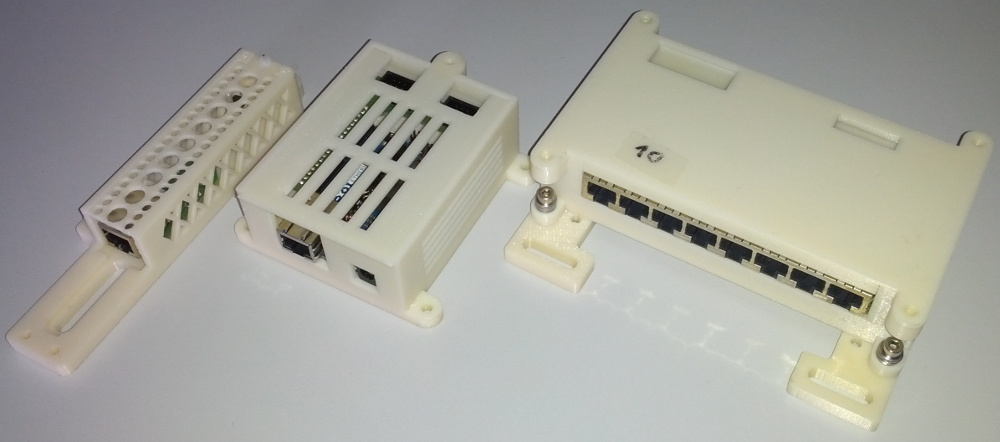
\includegraphics[width=\textwidth]{img/cases.jpg}
  \caption{3D printed casings. Left: temperature board casing, middle: ethernet board casing, right: collector board casing. The casing for the humidity board is not shown, as it is similar to the one for the temperature sensor, but longer.}
	\label{fig:casings}
\end{figure}
Casings for the electronic components were designed with 3D CAD software and then printed with the department's 3D printer. The 3D
files of each case can be found in our GIT repository. Figure \ref{fig:casings} shows the completed cases with circuit boards inside.
\paragraph{casings for the sensors}\hspace{1cm}\\
The casings for the sensor boards were designed to protect the sensors from being damaged, as well as to provide a convenient way of
mounting them on ITEM compatible aluminium profiles. The casing walls have a mesh structure, to allow a maximum air exchange aound the
sensor. To prevent damage of the sensor board caused by the ethernet cable, a strain-relief is also featured. The original design and
idea for the sensor casings was done by Tobias Lins.
\paragraph{Casings for the control units}\hspace{1cm}\\
We also designed cases for the ethernet and collector boards, to be able to mount them in an easy and compact manner.\\
Cases for the collector board were designed to be stackable. This works well with the I2C chaining feature, as to extend the sensor network,
only a new collector board has to be placed on top of the stack. The I2C plug can then be connected to the socket of the topmost board, and provides
communication and power to the new board.
%%%%%%%%%%%%%%%%%%%%%%%%%%%%%%%%%%%%%%%%%%%%%%%%%%%%%%%%%%%%%%%
\section{Installation}
\paragraph{Sensor distribution}\hspace{1cm}\\
In total we installed 42 temperature sensors and 2 humidity sensors inside the field
cage of the nEDM experiment setup. For convenient cable routing, we used
two control stations, each consisting out of three stacked collector boards and one
ethernet board. One of the control station is placed on the ceiling of the
topmost floor and the other one is placed near the ground in the lowest floor. We tried
to distribute the sensors evenly in the field cace. However, most
of the sensors were placed on the walls and ceilings of the individual floors. Figure
\ref{fig:install} shows the approximate distribution of sensors and control starions.\\
The two control stations feature sockets for 48 sensors, as we currently only use 44,
the remaining four sockets can be used, to connect additional sensors on demand\footnote{Note, that
the system is Plug and Play. This means the sensors may be connected and disconnected
while the system is running}.\\
\paragraph{Cable routing}\hspace{1cm}\\
We attached two unique identifier tags to each cable, connecting a sensor to a collector
board. This ID specifies, to which collector board and to which exact socket,
the cable should be connected. For example, the ID 'B013S0' means, that the cable should
be connected to collector board number 13 in the leftmost socket.\\
The cables leading to sensors, were collected in cable channels where possible and otherwise
fastened with cable straps to the cage skeleton.\\
Figure \ref{fig:control_unit} shows an installed control station with connected cables to
the individual sensors. In this case the powersupply is a 9V switching powersupply, connected
to one of the collector boards. The integrated coltage regulator of this board then creates
a 5V output, which drives all three collector boards via the I2C connection.
\begin{figure}
	\centering
	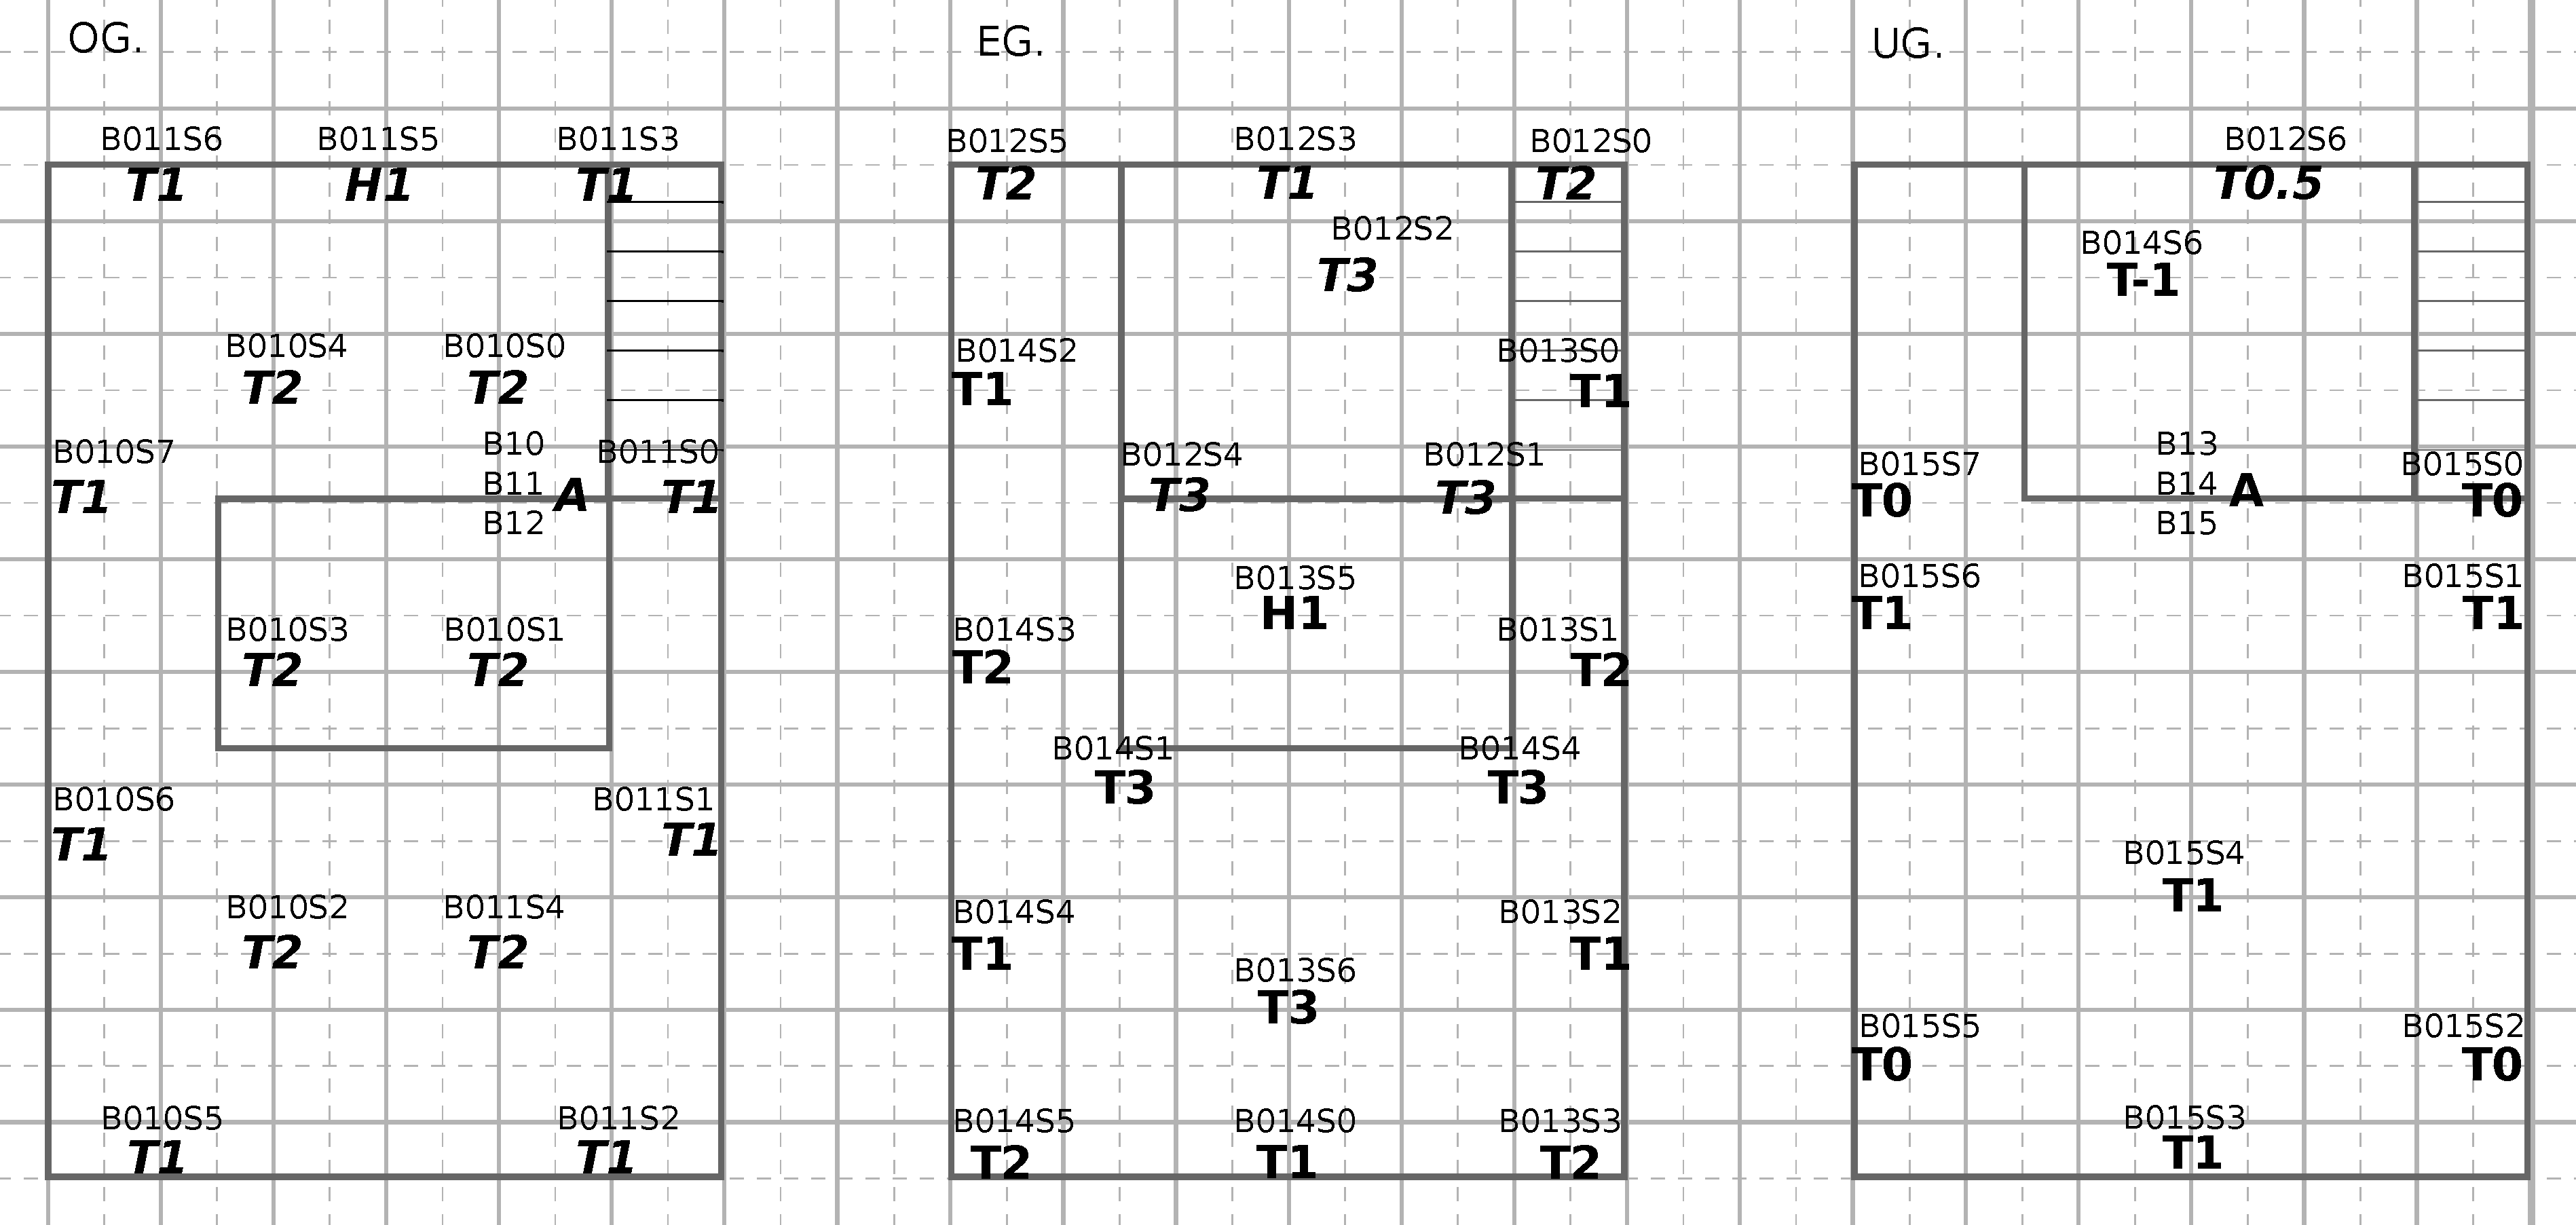
\includegraphics[width=\textwidth]{img/installPlan.pdf}
  \caption{Approximate sensor distribution in the field cage.}
	\label{fig:install}
\end{figure}
%%%%%%%%%%%%%%%%%%%%%%%%%%%%%%%%%%%%%%%%%%%%%%%%%%%%%%%%%%%%%%%
\section{Problems}
\subsection{Squid magnetic field measurement}
To detect possible magnetic interference of our sensor network with the nEDM experiment,
we performed two measurements, where
we placed 10 sensors and 6 collector boards inside the magnetically shielded room and performed
magnetic field measurements using a squid magnetometer. However both our measurements were
influenced by time dependant noise, which made the results not trustworthy.
\subsection{Crash after long uptime}
\paragraph{The problem}\hspace{1cm}\\
The software on the ethernet board currently contains a bug, which causes the board to
crash at semi-random times. As a result the ethernet board becomes completely inoperable.
The occurence of this problem is dependent on the configured sampling rate. At a sampling
interval of $5\,s$ it occurs after about 8 hours, at $\approx0.6\,s$ it occurs already after about
2 hours. Due to the random nature however, these time values represent mean values based on
observations.\\
After debugging, we found out, that the program is always crashing in the function
\texttt{net\_sendResultToDB(struct dummy\_packet *packets, uint8\_t board\_addr)}. We also found out, that the first part of the function executes correctly:
\definecolor{mygreen}{rgb}{0,0.6,0}
\lstdefinestyle{customc}{
  belowcaptionskip=1\baselineskip,
  breaklines=true,
  %frame=L,
  %xleftmargin=\parindent,
  language=C,
  showstringspaces=false,
  basicstyle=\footnotesize\ttfamily,
  %keywordstyle=\bfseries\color{green!40!black},
  %commentstyle=\itshape\color{purple!40!black},
  keywordstyle=\bfseries\color{mygreen},
  commentstyle=\itshape\color{blue},
  identifierstyle=\color{black},
  stringstyle=\color{red}
}
\lstset{style=customc}
\begin{lstlisting}[language=C, framextopmargin=10pt, framexbottommargin=10pt]
void net_sendResultToDB(struct dummy_packet *packets, uint8_t board_addr){
  // Sends a set of 8 measurement results to the couchdb database
  int8_t sensor_index;
  int8_t comma_flag = 0;
  int16_t value;
  uint16_t len=0;
  PORTB &= ~(1<<PB1);
  PORTD &= ~(1<<PD5);
  if( W5100.readSnSR(DB_CLIENT_SOCK) != SnSR::ESTABLISHED ){
    if(!connect_db(cfg.port+1)){
      return;
    }
  }
  // CRASH OCCURS SOMEWHERE AFTER THIS LINE:
  // Calculate length for the JSON header:
  for (sensor_index=0; sensor_index<8; sensor_index++){
    if(packets[sensor_index].header.error && packets[sensor_index].header.connected){
      // We do not send data, which might have an error
      continue;
    }
    if(packets[sensor_index].header.connected){
      switch(packets[sensor_index].header.type){
        case PACKET_TYPE_TSIC:
...
...
\end{lstlisting}
However we did not have enough time to exactly locate the problematic code.
\paragraph{The workaround}\hspace{1cm}\\
We implemented a workaround for this problem, using the integrated watchdog
timer (WDT) of the atmega88. This is a independent timer of the
controller, which can be reset via software. If a overflow of this thimer occurs,
a complete system reset of the chip will be performed. In our configuration, we
trigger a timer reset of the WDT on specific points during program execution.
If however the mentioned bug occurs, the program will hang and after a timeout
a system reset will occur. This can only be seen as a temporary solution, as
the bug still exists and timing of the measurement interval will not be right
for one measurement, as a crash might cause a blackout for up to 15 seconds.
\paragraph{Further debuging ideas}\hspace{1cm}\\
While debugging, we found out, that printing debug information over the USART
interface will heavily extend the time until the bug appears, so this is not a
good option for debugging the code. We had the most success, to locate the bug,
by changing the state of LEDs or other GPIOs at differend code locations. After
the system has crashed, we could just look at the LEDs or measure the voltage on
GPIO pins to see which line was still executed.
\subsection{Minor problems}
\subsubsection{Range of I2C}
In the design phase, we decided to use I2C for communication between
the collectorboards. This decision was made, because I2C features clock
extension and is flexible with regards to connecting new bus participants.\\
The drawback of this protocol however is, that it is not suitable for long
range communication, due to the pullup resistors, which allow dominant
bits. It would be possible to transfer I2C signals over a CAN physical layer
network, to increase range, however we did not implement this, due to
cost and complexity savings.\\
During deployment, we realized, that this is a weak point of our sensor
network, as we were limited to star shaped network topologies. In the case
for the nEDM experiment, this problem was not severe, as we only needed
two control points to conveniently route cables to all sensors from there.
So we used two ethernet boards, which was still more efficient in terms
of total cost, than using a CAN network.\\
However for bigger networks this would represent a drawback.
\subsubsection{Plug and Play with I2C}
Due to the many different bus states, and undefined behavior, when bus
participants are connected / disconnected during bus transactions, it was
very difficult to allow plug and play of collector boards on the I2C bus.\\
The current implementation works versy stable, however we can not guarantee
safe operation, when the device configuration changes during runtime, even though
we did not observe a crash in our tests.\\
This problem does not affect normal operation, as in the current setup in the
nEDM experiment, no collector boards will be added or removed during runtime
\footnote{Note that Plug and Play for the individual sensors works perfectly}.
If collectorboards are changed, a power cycle might have to be performed, if
the network freezes.
\subsubsection{Low fault tolerance of I2C}
Due to the nature of the bus, one failing I2C bus participant might be able to
block the whole bus, rendering the whole network unusable\footnote{Note that this
might happen, when the microcontroller is connected to a USBasp programmer, which
is not connected to a computer.}.
%%%%%%%%%%%%%%%%%%%%%%%%%%%%%%%%%%%%%%%%%%%%%%%%%%%%%%%%%%%%%%%
\section{Developing / Extending}
The following are tips for developers, which might me useful, when extending
the sensor network:
\begin{itemize}
\item To prevent EEPROM from being corrupted on power cycles, the AVR
  integrated brownout detection should be enabled.
\item To allow EEPROM stroage to stay intact after reprogramming, set the
  corresponding fuse bit.
\item To not overload the voltage regulator, especially when driving multiple
  boards one should consider, that a significant portion of power is used to
  drive LEDs ($\approx20\,\mathrm{mA}$ per LED). So turning the LEDs off during
  normal operation will prevent overheating.
\item When debugging and programming devices of the sensor network, one has to
  be very careful, to not provide different power sources, as this might cause
  unexpected results, which can lead to damage of the sensor network, as well
  ass connected computers. By default the USBasp programmer provides the system
  with 5V power.
\item As Arduino fuses are not possible to be programmed via the default Arduino
  programmer (using the Arduino bootloader), we removed the bootloader and use
  the ISP connector for programming (see section \ref{chap:isp}).
\item Our makefiles currently do not support automatic detection of
  file dependencies, and source files to be compiled. All source files have to
  be specified explicitly and if changes to header files are made, a 'make clean'
  should be performed before compiling the program.
\item Be careful, when using the USART line or similar for generating debugging
  output. Transmitting debugging information takes relatively long time and might
  influence the system heavily, especially, when debugging timing critical code.
  LEDs or GPIO pins with an oscilloscope provide a faster but more complex way for debugging.
\end{itemize}
%###############################################################
\chapter{References}
%\renewcommand\refname{\vskip -1cm}
%\bibliographystyle{abbrv}
\bibliographystyle{plain}
\begingroup
\def%###############################################################
\chapter*#1{}
\bibliography{bib}
\endgroup
%\bibliography{bib}
\nocite{*}

\begin{appendices}
%###############################################################
\chapter{Board Schematics}
\begin{figure}[Hh!]
	\centering
	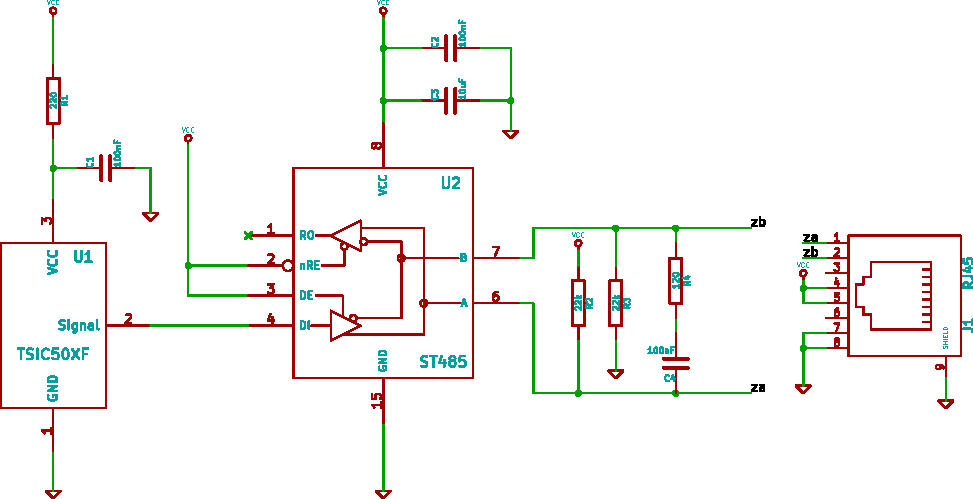
\includegraphics[width=0.7\textwidth]{img/schem_temperature_board.pdf}
	\caption{Temperature board schematic. The Impedance adjustor circuit, R4 and C4 is not required to be populated, as we only transmit data.}
	\label{fig:schem_temp}
\end{figure}
\begin{figure}[Hh!]
	\centering
	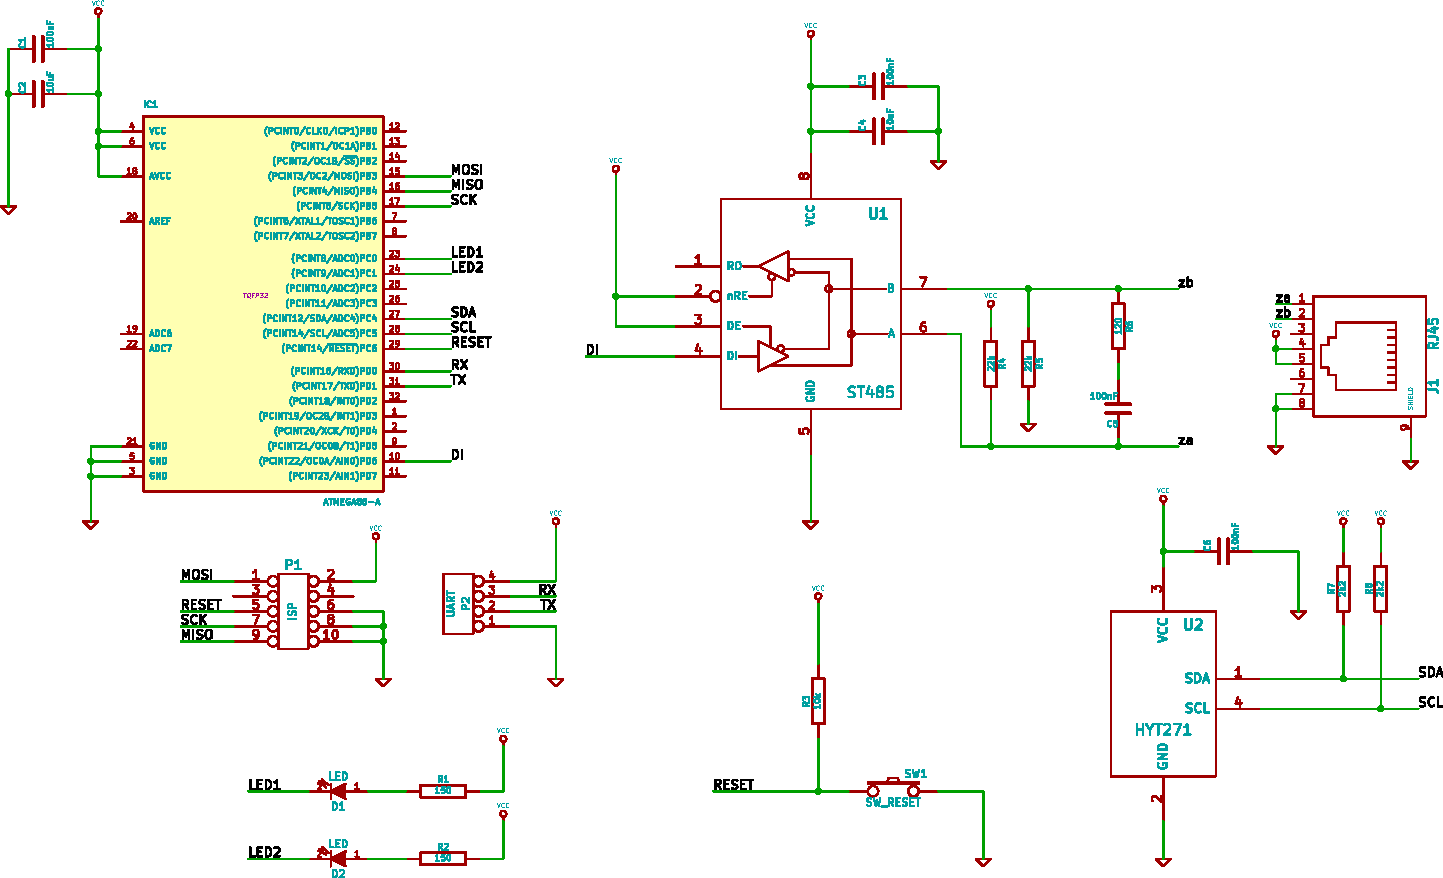
\includegraphics[width=0.9\textwidth]{img/schem_humidity_board.pdf}
	\caption{Humidity board schematic}
	\label{fig:schem_hum}
\end{figure}
\begin{figure}
	\centering
	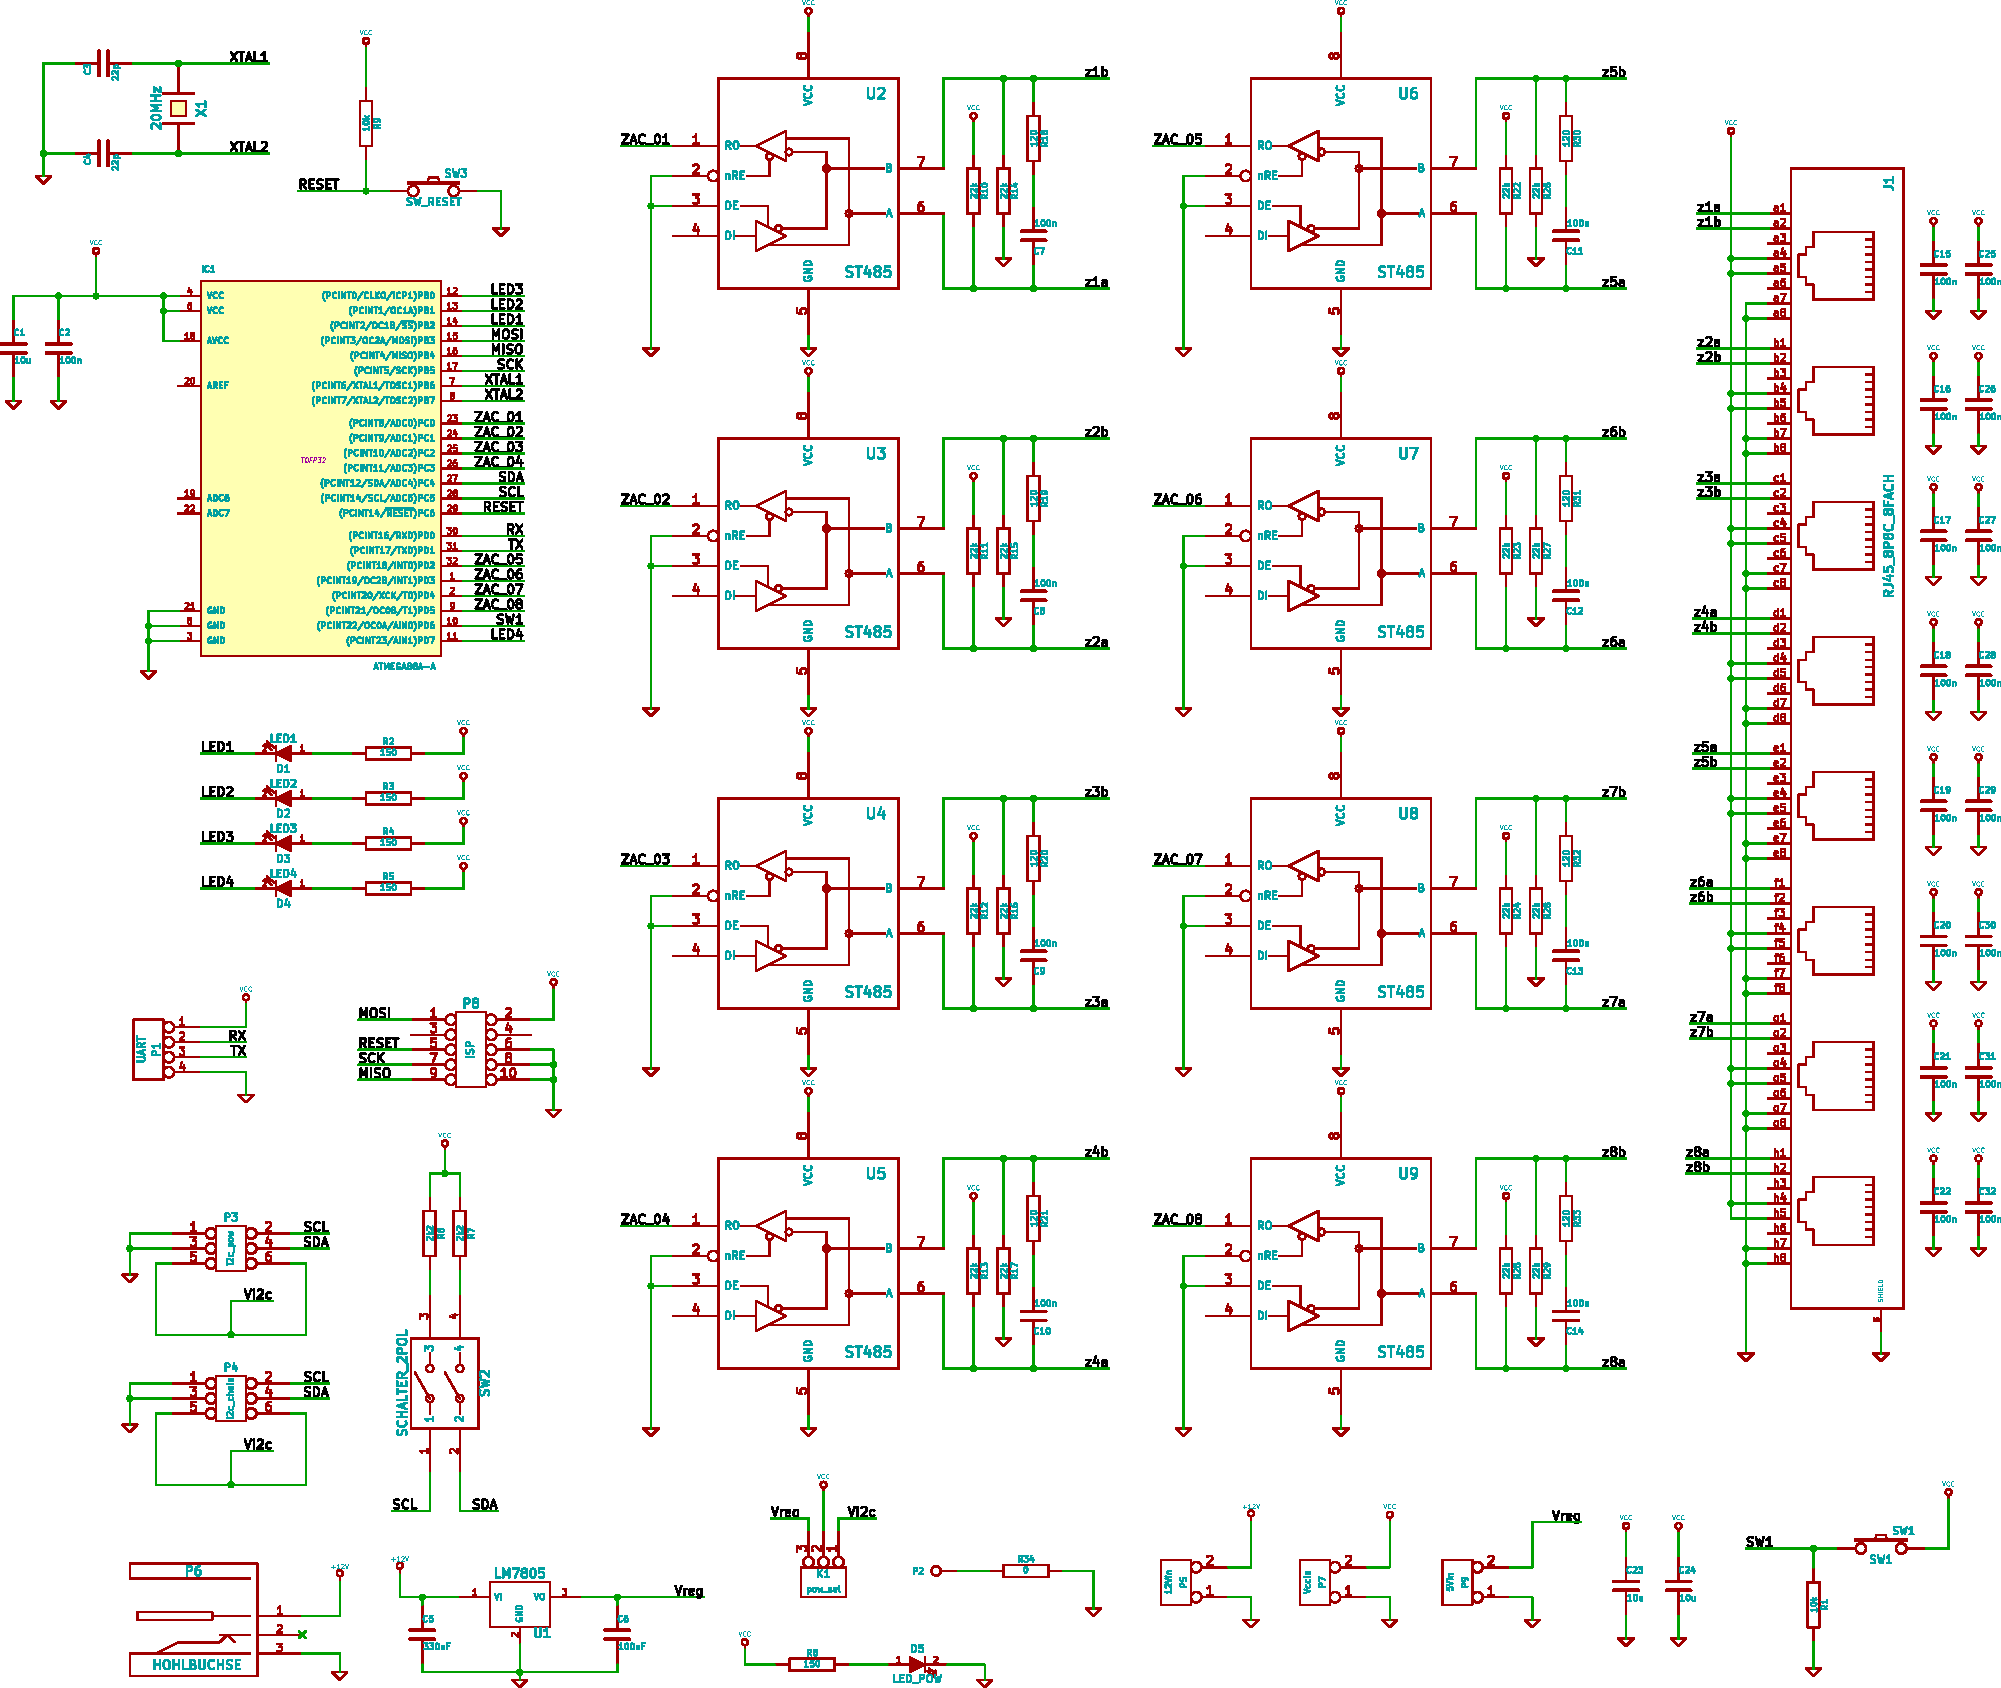
\includegraphics[width=1\textwidth]{img/schem_collector_board.pdf}
	\caption{Collector board schematic}
	\label{fig:schem_collect}
\end{figure}
%###############################################################
\chapter{Board PCB layout}
\begin{figure}[Hh!]
	\centering
	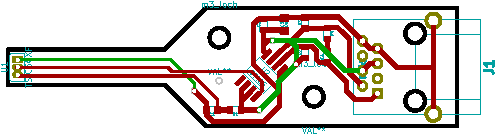
\includegraphics[width=0.7\textwidth]{img/boards/temperature_kicad.pdf}
	\caption{Temperature printed circuit board schematic. Ground planes are not displayed.}
	\label{fig:pcb_temp}
\end{figure}
\begin{figure}[Hh!]
	\centering
	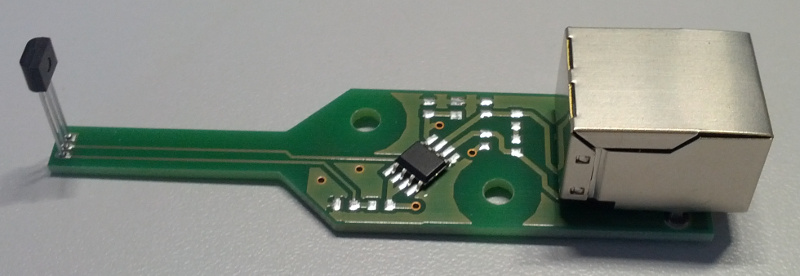
\includegraphics[width=0.7\textwidth]{img/boards/temperature_pcp.jpg}
	\caption{Temperature printed circuit board. Components not completely soldered yet.}
	\label{fig:soldered_temp}
\end{figure}
\begin{figure}[Hh!]
	\centering
	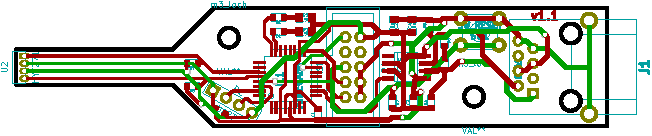
\includegraphics[width=0.9\textwidth]{img/boards/humidity_kicad.pdf}
	\caption{Humidity printed circuit board schematic. Ground planes are not displayed.}
	\label{fig:pcb_hum}
\end{figure}
\begin{figure}[Hh!]
	\centering
	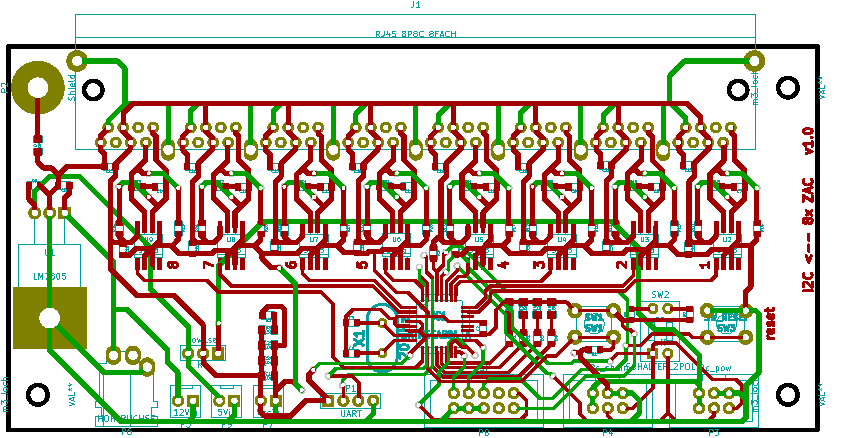
\includegraphics[height=0.7\textwidth, angle=270]{img/boards/collector_kicad.pdf}
	\caption{Collector board printed circuit board schematic. Ground planes are not displayed.}
	\label{fig:pcb_collector} %FIXME: add reference in text
\end{figure}
\begin{figure}[Hh!]
	\centering
	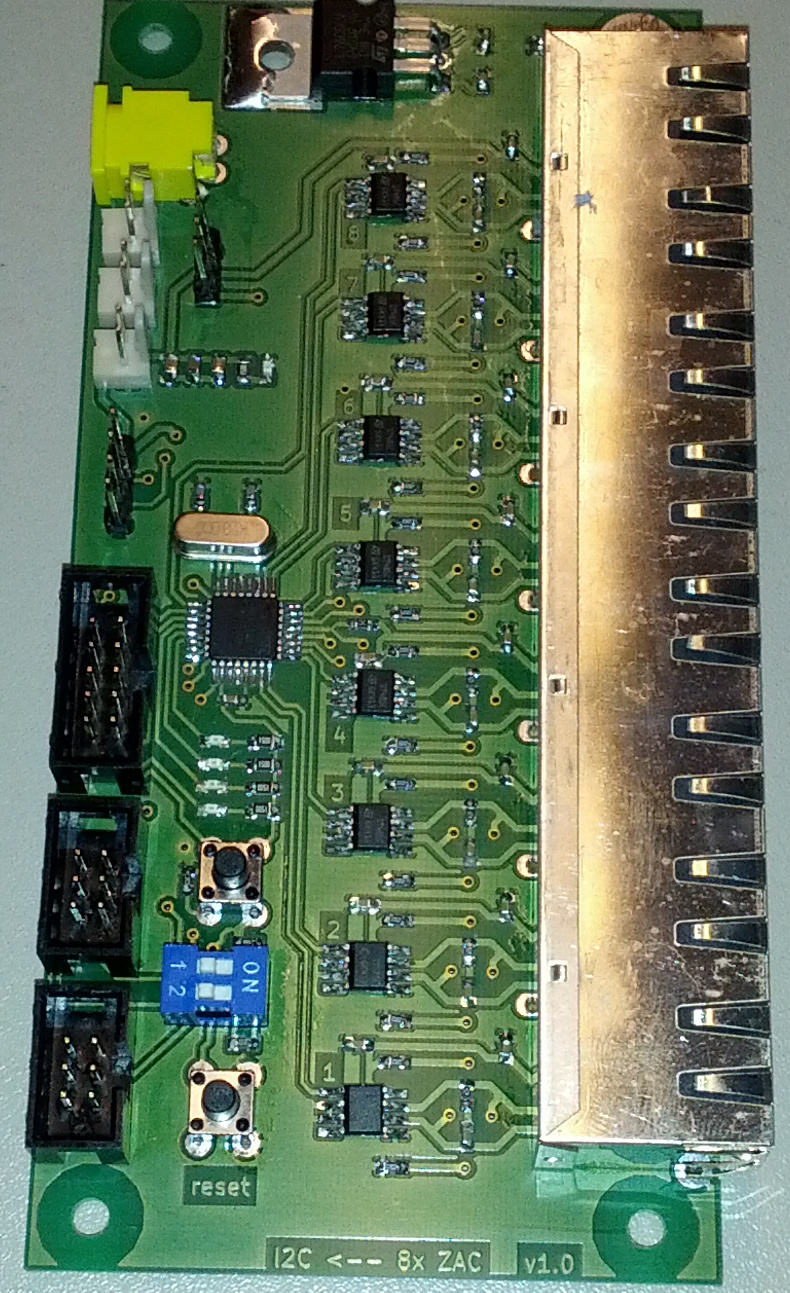
\includegraphics[width=0.4\textwidth]{img/boards/collector_complete.jpg}
	\caption{Collector printed circuit board, completely soldered.}
	\label{fig:soldered_col}
\end{figure}
\begin{figure}[Hh!]
	\centering
	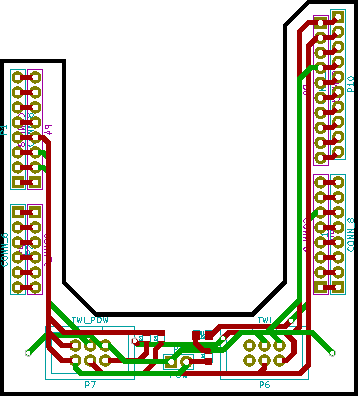
\includegraphics[width=0.4\textwidth]{img/boards/arduino_kicad.pdf}
	\caption{Arduino adapter printed circuit board schematic. Ground planes are not displayed.}
	\label{fig:pcb_arduino} 
\end{figure}

%###############################################################
\chapter{Deployment images}
\begin{figure}[Hh!]
	\centering
	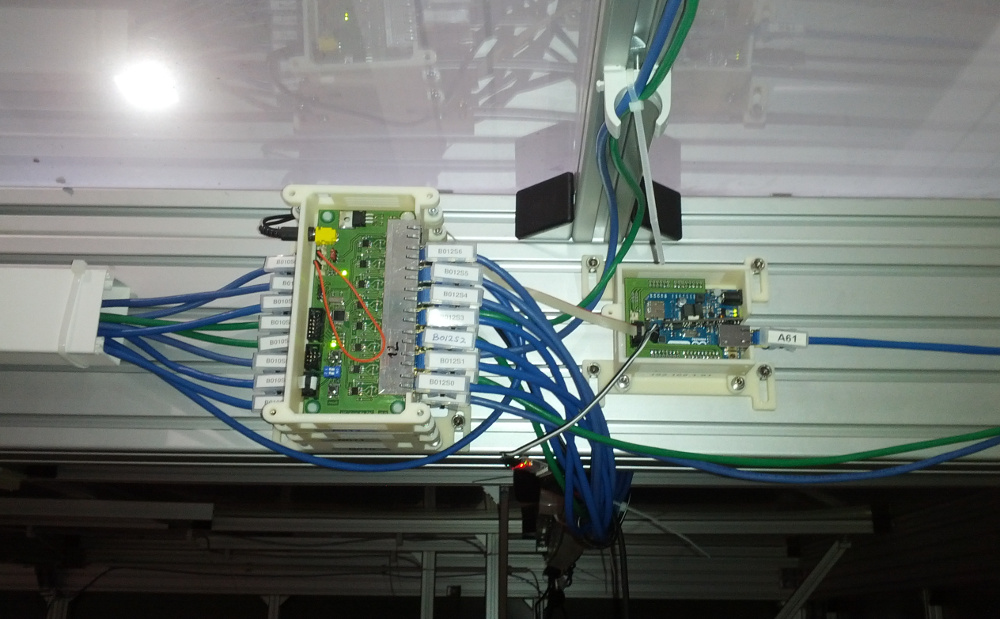
\includegraphics[width=0.94\textwidth]{img/control_unit.jpg}
	\caption{One of the two installed control units, consisting of three stacked collector boards and one ethernet board. The lids of the casings are removed here. Every cable to a sensor is marked with an unique identifier.}
	\label{fig:control_unit} %FIXME: add reference in text
\end{figure}
\end{appendices}

\end{document}
